\documentclass[]{book}
\usepackage{lmodern}
\usepackage{amssymb,amsmath}
\usepackage{ifxetex,ifluatex}
\usepackage{fixltx2e} % provides \textsubscript
\ifnum 0\ifxetex 1\fi\ifluatex 1\fi=0 % if pdftex
  \usepackage[T1]{fontenc}
  \usepackage[utf8]{inputenc}
\else % if luatex or xelatex
  \ifxetex
    \usepackage{mathspec}
  \else
    \usepackage{fontspec}
  \fi
  \defaultfontfeatures{Ligatures=TeX,Scale=MatchLowercase}
\fi
% use upquote if available, for straight quotes in verbatim environments
\IfFileExists{upquote.sty}{\usepackage{upquote}}{}
% use microtype if available
\IfFileExists{microtype.sty}{%
\usepackage{microtype}
\UseMicrotypeSet[protrusion]{basicmath} % disable protrusion for tt fonts
}{}
\usepackage[margin=1in]{geometry}
\usepackage{hyperref}
\hypersetup{unicode=true,
            pdftitle={Math Prefresher for Political Scientists},
            pdfauthor={Shiro Kuriwaki and Yon Soo Park},
            pdfborder={0 0 0},
            breaklinks=true}
\urlstyle{same}  % don't use monospace font for urls
\usepackage{natbib}
\bibliographystyle{apalike}
\usepackage{color}
\usepackage{fancyvrb}
\newcommand{\VerbBar}{|}
\newcommand{\VERB}{\Verb[commandchars=\\\{\}]}
\DefineVerbatimEnvironment{Highlighting}{Verbatim}{commandchars=\\\{\}}
% Add ',fontsize=\small' for more characters per line
\usepackage{framed}
\definecolor{shadecolor}{RGB}{248,248,248}
\newenvironment{Shaded}{\begin{snugshade}}{\end{snugshade}}
\newcommand{\KeywordTok}[1]{\textcolor[rgb]{0.13,0.29,0.53}{\textbf{#1}}}
\newcommand{\DataTypeTok}[1]{\textcolor[rgb]{0.13,0.29,0.53}{#1}}
\newcommand{\DecValTok}[1]{\textcolor[rgb]{0.00,0.00,0.81}{#1}}
\newcommand{\BaseNTok}[1]{\textcolor[rgb]{0.00,0.00,0.81}{#1}}
\newcommand{\FloatTok}[1]{\textcolor[rgb]{0.00,0.00,0.81}{#1}}
\newcommand{\ConstantTok}[1]{\textcolor[rgb]{0.00,0.00,0.00}{#1}}
\newcommand{\CharTok}[1]{\textcolor[rgb]{0.31,0.60,0.02}{#1}}
\newcommand{\SpecialCharTok}[1]{\textcolor[rgb]{0.00,0.00,0.00}{#1}}
\newcommand{\StringTok}[1]{\textcolor[rgb]{0.31,0.60,0.02}{#1}}
\newcommand{\VerbatimStringTok}[1]{\textcolor[rgb]{0.31,0.60,0.02}{#1}}
\newcommand{\SpecialStringTok}[1]{\textcolor[rgb]{0.31,0.60,0.02}{#1}}
\newcommand{\ImportTok}[1]{#1}
\newcommand{\CommentTok}[1]{\textcolor[rgb]{0.56,0.35,0.01}{\textit{#1}}}
\newcommand{\DocumentationTok}[1]{\textcolor[rgb]{0.56,0.35,0.01}{\textbf{\textit{#1}}}}
\newcommand{\AnnotationTok}[1]{\textcolor[rgb]{0.56,0.35,0.01}{\textbf{\textit{#1}}}}
\newcommand{\CommentVarTok}[1]{\textcolor[rgb]{0.56,0.35,0.01}{\textbf{\textit{#1}}}}
\newcommand{\OtherTok}[1]{\textcolor[rgb]{0.56,0.35,0.01}{#1}}
\newcommand{\FunctionTok}[1]{\textcolor[rgb]{0.00,0.00,0.00}{#1}}
\newcommand{\VariableTok}[1]{\textcolor[rgb]{0.00,0.00,0.00}{#1}}
\newcommand{\ControlFlowTok}[1]{\textcolor[rgb]{0.13,0.29,0.53}{\textbf{#1}}}
\newcommand{\OperatorTok}[1]{\textcolor[rgb]{0.81,0.36,0.00}{\textbf{#1}}}
\newcommand{\BuiltInTok}[1]{#1}
\newcommand{\ExtensionTok}[1]{#1}
\newcommand{\PreprocessorTok}[1]{\textcolor[rgb]{0.56,0.35,0.01}{\textit{#1}}}
\newcommand{\AttributeTok}[1]{\textcolor[rgb]{0.77,0.63,0.00}{#1}}
\newcommand{\RegionMarkerTok}[1]{#1}
\newcommand{\InformationTok}[1]{\textcolor[rgb]{0.56,0.35,0.01}{\textbf{\textit{#1}}}}
\newcommand{\WarningTok}[1]{\textcolor[rgb]{0.56,0.35,0.01}{\textbf{\textit{#1}}}}
\newcommand{\AlertTok}[1]{\textcolor[rgb]{0.94,0.16,0.16}{#1}}
\newcommand{\ErrorTok}[1]{\textcolor[rgb]{0.64,0.00,0.00}{\textbf{#1}}}
\newcommand{\NormalTok}[1]{#1}
\usepackage{longtable,booktabs}
\usepackage{graphicx,grffile}
\makeatletter
\def\maxwidth{\ifdim\Gin@nat@width>\linewidth\linewidth\else\Gin@nat@width\fi}
\def\maxheight{\ifdim\Gin@nat@height>\textheight\textheight\else\Gin@nat@height\fi}
\makeatother
% Scale images if necessary, so that they will not overflow the page
% margins by default, and it is still possible to overwrite the defaults
% using explicit options in \includegraphics[width, height, ...]{}
\setkeys{Gin}{width=\maxwidth,height=\maxheight,keepaspectratio}
\IfFileExists{parskip.sty}{%
\usepackage{parskip}
}{% else
\setlength{\parindent}{0pt}
\setlength{\parskip}{6pt plus 2pt minus 1pt}
}
\setlength{\emergencystretch}{3em}  % prevent overfull lines
\providecommand{\tightlist}{%
  \setlength{\itemsep}{0pt}\setlength{\parskip}{0pt}}
\setcounter{secnumdepth}{5}
% Redefines (sub)paragraphs to behave more like sections
\ifx\paragraph\undefined\else
\let\oldparagraph\paragraph
\renewcommand{\paragraph}[1]{\oldparagraph{#1}\mbox{}}
\fi
\ifx\subparagraph\undefined\else
\let\oldsubparagraph\subparagraph
\renewcommand{\subparagraph}[1]{\oldsubparagraph{#1}\mbox{}}
\fi

%%% Use protect on footnotes to avoid problems with footnotes in titles
\let\rmarkdownfootnote\footnote%
\def\footnote{\protect\rmarkdownfootnote}

%%% Change title format to be more compact
\usepackage{titling}

% Create subtitle command for use in maketitle
\newcommand{\subtitle}[1]{
  \posttitle{
    \begin{center}\large#1\end{center}
    }
}

\setlength{\droptitle}{-2em}
  \title{Math Prefresher for Political Scientists}
  \pretitle{\vspace{\droptitle}\centering\huge}
  \posttitle{\par}
  \author{Shiro Kuriwaki and Yon Soo Park}
  \preauthor{\centering\large\emph}
  \postauthor{\par}
  \predate{\centering\large\emph}
  \postdate{\par}
  \date{2018-06-19}

\usepackage{booktabs}

\usepackage{epsfig}
\usepackage{epstopdf}
\usepackage{rotate}
\usepackage{graphicx}
\usepackage{hyperref}
\usepackage{alphalph}
\usepackage{caption}
\usepackage[hang,flushmargin]{footmisc}
\usepackage{framed}
\usepackage{xcolor}
\usepackage{verbatim} 

\usepackage{bm}
\setcounter{MaxMatrixCols}{20}
\newcommand{\Var}{\mathrm{Var}}
\newcommand{\SD}{\mathrm{SD}}
\newcommand{\Cov}{\mathrm{Cov}}
\newcommand{\fx}{f({\bf x})}
\newcommand\R{{\textsf R~}}
\newcommand\Rst{\textsf{RStudio}}

\oddsidemargin=0in
\evensidemargin=0in
\textwidth=6.5in
\topmargin=0in
\headsep=.25in
\headheight=.25in
\textheight=9.25in
\topskip=0in
\voffset=-0.5in
\epsfxsize=1in

\usepackage{amsthm}
\newtheorem{theorem}{Theorem}[chapter]
\newtheorem{lemma}{Lemma}[chapter]
\theoremstyle{definition}
\newtheorem{definition}{Definition}[chapter]
\newtheorem{corollary}{Corollary}[chapter]
\newtheorem{proposition}{Proposition}[chapter]
\theoremstyle{definition}
\newtheorem{example}{Example}[chapter]
\theoremstyle{definition}
\newtheorem{exercise}{Exercise}[chapter]
\theoremstyle{remark}
\newtheorem*{remark}{Remark}
\newtheorem*{solution}{Solution}
\begin{document}
\maketitle

{
\setcounter{tocdepth}{1}
\tableofcontents
}
\chapter{About this Booklet}\label{about-this-booklet}

The documents in this booklet are the product of generations of Math
(P)refresher Instructors: Curt Signorino 1996-1997; Ken Scheve
1997-1998; Eric Dickson 1998-2000; Orit Kedar 1999; James Fowler
2000-2001; Kosuke Imai 2001-2002; Jacob Kline 2002; Dan Epstein 2003;
Ben Ansell 2003-2004; Ryan Moore 2004-2005; Mike Kellermann 2005-2006;
Ellie Powell 2006-2007; Jen Katkin 2007-2008; Patrick Lam 2008-2009;
Viridiana Rios 2009-2010; Jennifer Pan 2010-2011; Konstantin Kashin
2011-2012; Sol'\{e\} Prillaman 2013; Stephen Pettigrew 2013-2014; Anton
Strezhnev 2014-2015; Mayya Komisarchik 2015-2016; Connor Jerzak
2016-2017; Shiro Kuriwaki 2017-2018; Yon Soo Park 2018-

\chapter{Linear Algebra}\label{linear-algebra}

Topics: \(\bullet\) Working with Vectors \(\bullet\) Linear Independence
\(\bullet\) Basics of Matrix Algebra \(\bullet\) Square Matrices
\(\bullet\) Linear Equations \(\bullet\) Systems of Linear Equations
\(\bullet\) Systems of Equations as Matrices \(\bullet\) Solving
Augmented Matrices and Systems of Equations \(\bullet\) Rank \(\bullet\)
The Inverse of a Matrix \(\bullet\) Inverse of Larger Matrices

Much of the material and examples for this lecture are taken from Gill
(2006) \emph{Essential Mathematics for Political and Social Scientists},
Simon \& Blume (1994) \emph{Mathematics for Economists} and Kolman
(1993) \emph{Introductory Linear Algebra with Applications}.

\section{Working with Vectors}\label{working-with-vectors}

\textbf{Vector}: A vector in \(n\)-space is an ordered list of \(n\)
numbers. These numbers can be represented as either a row vector or a
column vector:
\[ {\bf v} \begin{pmatrix} v_1 & v_2 & \dots & v_n\end{pmatrix} , {\bf v} = \begin{pmatrix} v_1 \\ v_2 \\ \vdots \\ v_n \end{pmatrix}\]

We can also think of a vector as defining a point in \(n\)-dimensional
space, usually \({\bf R}^n\); each element of the vector defines the
coordinate of the point in a particular direction.

\textbf{Vector Addition and Subtraction}: If two vectors, \({\bf u}\)
and \({\bf v}\), have the same length (i.e.~have the same number of
elements), they can be added (subtracted) together:
\[ {\bf u} + {\bf v} = \begin{pmatrix} u_1 + v_1 & u_2 + v_2 & \cdots & u_k + v_n \end{pmatrix}\]
\[ {\bf u} - {\bf v} = \begin{pmatrix} u_1 - v_1 & u_2 - v_2 & \cdots & u_k - v_n \end{pmatrix}\]

\textbf{Scalar Multiplication}: The product of a scalar \(c\) (i.e.~a
constant) and vector \({\bf v}\) is:\\
\[ c{\bf v} =  \begin{pmatrix} cv_1 & cv_2 & \dots & cv_n \end{pmatrix} \]

\textbf{Vector Inner Product}: The inner product (also called the dot
product or scalar product) of two vectors \({\bf u}\) and \({\bf v}\) is
again defined iff they have the same number of elements
\[ {\bf u} \cdot {\bf v} = u_1v_1 + u_2v_2 + \cdots + u_nv_n = \sum_{i = 1}^n u_iv_i\]
If \({\bf u} \cdot {\bf v} = 0\), the two vectors are orthogonal (or
perpendicular).

\textbf{Vector Norm}: The norm of a vector is a measure of its length.
There are many different ways to calculate the norm, but the most common
of is the Euclidean norm (which corresponds to our usual conception of
distance in three-dimensional space):
\[ ||{\bf v}|| = \sqrt{{\bf v}\cdot{\bf v}} = \sqrt{ v_1v_1 + v_2v_2 + \cdots + v_nv_n}\]

\section{Linear Independence}\label{linear-independence}

\textbf{Linear combinations}: The vector \({\bf u}\) is a linear
combination of the vectors \({\bf v}_1, {\bf v}_2, \cdots , {\bf v}_k\)
if \[{\bf u} = c_1{\bf v}_1 + c_2{\bf v}_2 +  \cdots + c_k{\bf v}_k\]

\textbf{Linear independence}: A set of vectors
\({\bf v}_1, {\bf v}_2, \cdots , {\bf v}_k\) is linearly independent if
the only solution to the equation
\[c_1{\bf v}_1 + c_2{\bf v}_2 +  \cdots + c_k{\bf v}_k = 0\] is
\(c_1 = c_2 = \cdots = c_k = 0\). If another solution exists, the set of
vectors is linearly dependent.

A set \(S\) of vectors is linearly dependent iff at least one of the
vectors in \(S\) can be written as a linear combination of the other
vectors in \(S\).

Linear independence is only defined for sets of vectors with the same
number of elements; any linearly independent set of vectors in
\(n\)-space contains at most \(n\) vectors.

Exercises: Are the following sets of vectors linearly independent?

\begin{enumerate}
        \item $${\bf v}_1 = \begin{pmatrix} 1 \\ 0 \\ 0 \end{pmatrix} , {\bf v}_2 = \begin{pmatrix} 1 \\ 0 \\ 1 \end{pmatrix} , {\bf v}_3 = \begin{pmatrix} 1 \\ 1 \\ 1 \end{pmatrix} $$ 
            \phantom{Yes}
        \item $${\bf v}_1 = \begin{pmatrix} 3 \\ 2 \\ -1 \end{pmatrix} , {\bf v}_2 = \begin{pmatrix} -2 \\ 2 \\ 4 \end{pmatrix} , {\bf v}_3 = \begin{pmatrix} 2 \\ 3 \\ 1 \end{pmatrix} $$ 
            \phantom{No. $-{\bf v}_1 - .5\cdot {\bf v}_2 + {\bf v}_3 = 0$}
\end{enumerate}

\section{Basics of Matrix Algebra}\label{basics-of-matrix-algebra}

\textbf{Matrix}: A matrix is an array of real numbers arranged in \(m\)
rows by \(n\) columns. The dimensionality of the matrix is defined as
the number of rows by the number of columns, \(m x n\).

\[{\bf A}=\begin{pmatrix}
            a_{11} & a_{12} & \cdots & a_{1n} \\
            a_{21} & a_{22} & \cdots & a_{2n} \\
            \vdots & \vdots & \ddots & \vdots \\
            a_{m1} & a_{m2} & \cdots & a_{mn}
        \end{pmatrix}\]

Note that you can think of vectors as special cases of matrices; a
column vector of length \(k\) is a \(k \times 1\) matrix, while a row
vector of the same length is a \(1 \times k\) matrix.

It's also useful to think of matrices as being made up of a collection
of row or column vectors. For example,
\[\bf A = \begin{pmatrix} {\bf a}_1 & {\bf a}_2 &  \cdots & {\bf a}_m \end{pmatrix}\]

\textbf{Matrix Addition}: Let \(\bf A\) and \(\bf B\) be two
\(m\times n\) matrices. \[{\bf A+B}=\begin{pmatrix}
            a_{11}+b_{11} & a_{12}+b_{12} & \cdots & a_{1n}+b_{1n} \\
            a_{21}+b_{21} & a_{22}+b_{22} & \cdots & a_{2n}+b_{2n} \\
            \vdots & \vdots  & \ddots & \vdots \\
            a_{m1}+b_{m1} & a_{m2}+b_{m2} & \cdots & a_{mn}+b_{mn}
        \end{pmatrix}\]

Note that matrices \({\bf A}\) and \({\bf B}\) must have the same
dimensionality, in which case they are \textbf{conformable for
addition}.

Example:
\[{\bf A}=\begin{pmatrix} 1 & 2 & 3 \\ 4 & 5 & 6 \end{pmatrix}, \qquad
            {\bf B}=\begin{pmatrix} 1 & 2 & 1 \\ 2 & 1 & 2 \end{pmatrix}\]
\[{\bf A+B}= \phantom{\begin{pmatrix} 2 & 4 & 4 \\ 6 & 6 & 8 \end{pmatrix}}\]

\textbf{Scalar Multiplication}: Given the scalar \(s\), the scalar
multiplication of \(s {\bf A}\) is \[ s {\bf A}=  s \begin{pmatrix}
            a_{11} & a_{12} & \cdots & a_{1n} \\
            a_{21} & a_{22} & \cdots & a_{2n} \\
            \vdots & \vdots & \ddots & \vdots \\
            a_{m1} & a_{m2} & \cdots & a_{mn}
        \end{pmatrix}
        = \begin{pmatrix}
            s a_{11} & s a_{12} & \cdots & s a_{1n} \\
            s a_{21} & s a_{22} & \cdots & s a_{2n} \\
            \vdots & \vdots & \ddots & \vdots \\
            s a_{m1} & s a_{m2} & \cdots & s a_{mn}
        \end{pmatrix}\]

Example:
\[s=2, \qquad {\bf A}=\begin{pmatrix} 1 & 2 & 3 \\ 4 & 5 & 6 \end{pmatrix}\]
\[s {\bf A} = \phantom{\begin{pmatrix} 2 & 4 & 6 \\ 8 & 10 & 12 \end{pmatrix}}\]

\textbf{Matrix Multiplication}: If \({\bf A}\) is an \(m\times k\)
matrix and \(\bf B\) is a \(k\times n\) matrix, then their product
\(\bf C = A B\) is the \(m\times n\) matrix where
\[c_{ij}=a_{i1}b_{1j}+a_{i2}b_{2j}+\cdots+a_{ik}b_{kj}\]

Examples:

\begin{enumerate}
        \item $\begin{pmatrix} a&b\\c&d\\e&f \end{pmatrix} \begin{pmatrix} A&B\\C&D \end{pmatrix}
            = \phantom{\begin{pmatrix} aA+bC&aB+bD\\cA+dC&cB+dD\\eA+fC&eB+fD \end{pmatrix}}$ 
        
        \item $\begin{pmatrix} 1&2&-1\\3&1&4 \end{pmatrix} \begin{pmatrix} -2&5\\4&-3\\2&1\end{pmatrix} = 
            \phantom{\begin{pmatrix} 1(-2)+2(4)-1(2)&1(5)+2(-3)-1(1)\\
                3(-2)+1(4)+4(2)&3(5)+1(-3)+4(1)\end{pmatrix} =
            \begin{pmatrix} 4&-2\\6&16\end{pmatrix}}$
    \end{enumerate}

Note that the number of columns of the first matrix must equal the
number of rows of the second matrix, in which case they are
\textbf{conformable for multiplication}. The sizes of the matrices
(including the resulting product) must be
\[(m\times k)(k\times n)=(m\times n)\]

Also note that if \textbf{AB} exists, \textbf{BA} exists only if
\(\dim({\bf A}) = m \times n\) and \(\dim({\bf B}) = n \times m\).

This does not mean that \textbf{AB} = \textbf{BA}. \textbf{AB} =
\textbf{BA} is true only in special circumstances, like when \({\bf A}\)
or \({\bf B}\) is an identity matrix, \({\bf A} = {\bf B}^{-1}\), or
\({\bf A} = {\bf B}\) and \textbf{A} is idempotent.

\textbf{Laws of Matrix Algebra}:

\begin{enumerate}
        \item \parbox[t]{1.5in}{Associative:} $\bf (A+B)+C = A+(B+C)$\\
            \parbox[t]{1.5in}{\quad}  $\bf (AB)C = A(BC)$
        \item \parbox[t]{1.5in}{Commutative:} $\bf A+B=B+A$
        \item \parbox[t]{1.5in}{Distributive:} $\bf A(B+C)=AB+AC$\\
            \parbox[t]{1.5in}{\quad}   $\bf (A+B)C=AC+BC$
\end{enumerate}

Commutative law for multiplication does not hold -- the order of
multiplication matters: \[\bf AB\ne BA\]

Example:
\[{\bf A}=\begin{pmatrix} 1&2\\-1&3\end{pmatrix}, \qquad {\bf B}=\begin{pmatrix} 2&1\\0&1\end{pmatrix}\]
\[{\bf AB}=\begin{pmatrix} 2&3\\-2&2\end{pmatrix}, \qquad {\bf BA}=\begin{pmatrix} 1&7\\-1&3\end{pmatrix}\]

\textbf{Transpose}: The transpose of the \(m\times n\) matrix \(\bf A\)
is the \(n\times m\) matrix \({\bf A}^T\) (also written \({\bf A}'\))
obtained by interchanging the rows and columns of \(\bf A\).

Examples:

\begin{enumerate}
        \item ${\bf A}=\begin{pmatrix} 4&-2&3\\0&5&-1\end{pmatrix}, \qquad {\bf A}^T=\begin{pmatrix} 4&0\\-2&5\\3&-1 \end{pmatrix}$
        \item ${\bf B}=\begin{pmatrix} 2\\-1\\3 \end{pmatrix}, \qquad {\bf B}^T=\begin{pmatrix} 2&-1&3\end{pmatrix}$
    \end{enumerate}

The following rules apply for transposed matrices:

\begin{enumerate}
        \item $({\bf A+B})^T = {\bf A}^T+{\bf B}^T$
        \item $({\bf A}^T)^T={\bf A}$
        \item $(s{\bf A})^T = s{\bf A}^T$
        \item $({\bf AB})^T = {\bf B}^T{\bf A}^T$; and by induction $({\bf ABC})^T = {\bf C}^T{\bf B}^T{\bf A}^T$
\end{enumerate}

Example of \(({\bf AB})^T = {\bf B}^T{\bf A}^T\):
\[{\bf A}=\begin{pmatrix} 1&3&2\\2&-1&3\end{pmatrix}, \qquad {\bf B}=\begin{pmatrix} 0&1\\2&2\\3&-1\end{pmatrix}\]
\[ ({\bf AB})^T = \left[ \begin{pmatrix} 1&3&2\\2&-1&3\end{pmatrix} \begin{pmatrix} 0&1\\2&2\\3&-1\end{pmatrix} \right]^T = \begin{pmatrix} 12&7\\5&-3 \end{pmatrix}\]
\[ {\bf B}^T{\bf A}^T= \begin{pmatrix} 0&2&3\\1&2&-1 \end{pmatrix}  \begin{pmatrix} 1&2\\3&-1\\2&3 \end{pmatrix} = \begin{pmatrix} 12&7\\5&-3 \end{pmatrix}\]

\section{Square Matrices}\label{square-matrices}

\textbf{Square} matrices have the same number of rows and columns; a
\(k \times k\) square matrix is referred to as a matrix of order \(k\).

The \textbf{diagonal} of a square matrix is the vector of matrix
elements that have the same subscripts. If \textbf{A} is a square matrix
of order \(k\), then its diagonal is
\([ a_{11}, a_{22}, \dots, a_{kk}]'\).

There are several important types of square matrices:

\begin{enumerate}
\def\labelenumi{\arabic{enumi}.}
\item
  \textbf{Identity Matrix}: The \(n\times n\) identity matrix
  \({\bf I}_n\) is the matrix whose diagonal elements are 1 and all
  off-diagonal elements are 0. Examples:
  \[ {\bf I}_2=\begin{pmatrix} 1&0\\0&1 \end{pmatrix}, \qquad {\bf I}_3=\begin{pmatrix} 1&0&0\\ 0&1&0\\ 
          0&0&1 \end{pmatrix}\]
\item
  \textbf{Symmetric Matrix}: A matrix \textbf{A} is symmetric if
  \({\bf A} = {\bf A}'\); this implies that \(a_{ij} = a_{ji}\) for all
  \(i\) and \(j\). Examples:
  \[ {\bf A} = \begin{pmatrix} 1&2\\2&1 \end{pmatrix} = {\bf A}', \qquad {\bf B} =\begin{pmatrix} 4&2&-1\\ 2&1&3\\
          -1&3&1 \end{pmatrix} = {\bf B}'\]
\item
  \textbf{Diagonal Matrix}: A matrix \textbf{A} is diagonal if all of
  its non-diagonal entries are zero; formally, if \(a_{ij} = 0\) for all
  \(i \neq j\) Examples:
  \[ {\bf A} = \begin{pmatrix} 1&0\\0&2 \end{pmatrix}, \qquad {\bf B} =\begin{pmatrix} 4&0&0\\ 0&1&0\\
          0&0&1 \end{pmatrix}\]
\item
  \textbf{Triangular Matrix}: A matrix is triangular one of two cases.
  If all entries below the diagonal are zero (\(a_{ij} = 0\) for all
  \(i > j\)), it is \textbf{upper triangular}. Conversely, if all
  entries above the diagonal are zero (\(a_{ij} = 0\) for all
  \(i < j\)), it is \textbf{lower triangular}.
\end{enumerate}

Examples:
\[ {\bf A}_{LT}= \begin{pmatrix} 1&0 & 0\\4&2&0\\-3 & 2 & 5 \end{pmatrix}, \qquad {\bf A}_{UT}=\begin{pmatrix} 1&7&-4\\ 0&3&9\\
0&0&-3 \end{pmatrix}\]

\section{Linear Equations}\label{linear-equations}

\textbf{Linear Equation}: \(a_1 x_1 + a_2 x_2 + \cdots + a_n x_n = b\)

\(a_i\) are parameters or coefficients. \(x_i\) are variables or
unknowns.

Linear because only one variable per term and degree is at most 1.

\begin{enumerate} 
        \item \parbox[t]{1.5in}{${\bf R}^2$: line} $x_2 = \frac{b}{a_2}-\frac{a_1}{a_2} x_1$
        \item \parbox[t]{1.5in}{${\bf R}^3$: plane} $x_3= \frac{b}{a_3}-\frac{a_1}{a_3} x_1-\frac{a_2}{a_3} x_2 $
        \item ${\bf R}^n$: hyperplane
    \end{enumerate}

\section{Systems of Linear Equations}\label{systems-of-linear-equations}

We are often interested in solving linear systems like\textbackslash{}

\[\begin{matrix}
            x  & - & 3y & = & -3\\
            2x & + &  y & = &  8
            \end{matrix}\]

\begin{comment}
        \parbox[t]{1in}{\includegraphics[angle=270, width = 1in]{linsys.eps}}
\end{comment}

More generally, we might have a system of \(m\) equations in \(n\)
unknowns

\[\begin{matrix}
            a_{11}x_1  & + & a_{12}x_2 & + & \cdots & + & a_{1n}x_n & = & b_1\\
            a_{21}x_1  & + & a_{22}x_2 & + & \cdots & + & a_{2n}x_n & = & b_2\\
            \vdots     &   &     &   & \vdots &   &     & \vdots & \\
            a_{m1}x_1  & + & a_{m2}x_2 & + & \cdots & + & a_{mn}x_n & = & b_m
            \end{matrix}\]

A \textbf{solution} to a linear system of \(m\) equations in \(n\)
unknowns is a set of \(n\) numbers \(x_1, x_2, \cdots, x_n\) that
satisfy each of the \(m\) equations.

\begin{enumerate} 
        \item ${\bf R}^2$: intersection of the lines. 
        \item ${\bf R}^3$: intersection of the planes.
        \item ${\bf R}^n$: intersection of the hyperplanes.
    \end{enumerate}

Example: \(x=3\) and \(y=2\) is the solution to the above \(2\times 2\)
linear system. Notice from the graph that the two lines intersect at
\((3,2)\).

Does a linear system have one, no, or multiple solutions? For a system
of 2 equations in 2 unknowns (i.e., two lines):

\begin{enumerate}
        \item \parbox[t]{1.5in}{One solution:} The lines intersect at exactly one point.
        \item \parbox[t]{1.5in}{No solution:}  The lines are parallel.
        \item \parbox[t]{1.5in}{Infinite solutions:} The lines coincide.
\end{enumerate}

Methods to solve linear systems:

\begin{enumerate}
\def\labelenumi{\arabic{enumi}.}
\tightlist
\item
  Substitution
\item
  Elimination of variables
\item
  Matrix methods
\end{enumerate}

\section{Systems of Equations as
Matrices}\label{systems-of-equations-as-matrices}

Matrices provide an easy and efficient way to represent linear systems
such as \[\begin{matrix}
        a_{11}x_1  & + & a_{12}x_2 & + & \cdots & + & a_{1n}x_n & = & b_1\\
        a_{21}x_1  & + & a_{22}x_2 & + & \cdots & + & a_{2n}x_n & = & b_2\\
        \vdots     &   &     &   & \vdots &   &     & \vdots & \\
        a_{m1}x_1  & + & a_{m2}x_2 & + & \cdots & + & a_{mn}x_n & = & b_m
        \end{matrix}\]

as \[{\bf A x = b}\] where

\begin{enumerate}

\item The $m \times n$ \textbf{coefficient matrix} ${\bf A}$ is an array of $m n$  real numbers arranged in $m$ rows by $n$ columns:
            $${\bf A}=\begin{pmatrix}
            a_{11} & a_{12} & \cdots & a_{1n} \\
            a_{21} & a_{22} & \cdots & a_{2n} \\
            \vdots &  & \ddots & \vdots \\
            a_{m1} & a_{m2} & \cdots & a_{mn}
            \end{pmatrix}$$

        \item The unknown quantities are represented by the vector ${\bf x}=\begin{pmatrix} x_1\\x_2\\\vdots\\x_n \end{pmatrix}$.
        \item The right hand side of the linear system is represented by the vector ${\bf b}=\begin{pmatrix} b_1\\b_2\\\vdots\\b_m \end{pmatrix}$.
    \end{enumerate}

\textbf{Augmented Matrix}: When we append \(\bf b\) to the coefficient
matrix \(\bf A\), we get the augmented matrix
\(\widehat{\bf A}=[\bf A | b]\) \[\begin{pmatrix}
            a_{11} & a_{12} & \cdots & a_{1n} & | & b_1\\
            a_{21} & a_{22} & \cdots & a_{2n} & | & b_2\\
            \vdots &  & \ddots & \vdots & | & \vdots\\
            a_{m1} & a_{m2} & \cdots & a_{mn} & | & b_m
            \end{pmatrix}\]

\section{Finding Solutions to Augmented Matrices and Systems of
Equations}\label{finding-solutions-to-augmented-matrices-and-systems-of-equations}

\textbf{Row Echelon Form}: Our goal is to translate our augmented matrix
or system of equations into row echelon form. This will provide us with
the values of the vector \textbf{x} which solve the system. We use the
row operations to change coefficients in lower triangle of the augmented
matrix to 0. An augmented matrix of the form

\[\begin{pmatrix}
            \fbox{$a'_{11}$}& a'_{12} & a'_{13}& \cdots & a'_{1n} & | & b'_1\\
            0 & \fbox{$a'_{22}$} & a'_{23}& \cdots & a'_{2n} & | & b'_2\\
            0 & 0 & \fbox{$a'_{33}$}& \cdots & a'_{3n} & | & b'_3\\
            0 & 0 &0 & \ddots & \vdots  & | & \vdots \\
            0 & 0 &0 &0 & \fbox{$a'_{mn}$} & | & b'_m
            \end{pmatrix}\]

is said to be in row echelon form --- each row has more leading zeros
than the row preceding it.

\textbf{Reduced Row Echelon Form}: We can go one step further and put
the matrix into reduced row echelon form. Reduced row echelon form makes
the value of \textbf{x} which solves the system very obvious. For a
system of \(m\) equations in \(m\) unknowns, with no all-zero rows, the
reduced row echelon form would be

\[\begin{pmatrix}
            \fbox{$1$}  &  0 &   0 &    0  &   0 & | & b^*_1\\
            0  &  \fbox{$1$} &   0 &    0  &   0 & | & b^*_2\\
            0  &  0 &   \fbox{$1$} &    0  &   0 & | & b^*_3\\
            0  &  0 &   0 &\ddots &   0 & | &\vdots\\
            0  &  0 &   0 &    0  &   \fbox{$1$} & | & b^*_m
            \end{pmatrix}\]

\textbf{Gaussian and Gauss-Jordan elimination}: We can conduct
elementary row operations to get our augmented matrix into row echelon
or reduced row echelon form. The methods of transforming a matrix or
system into row echelon and reduced row echelon form are referred to as
Gaussian elimination and Gauss-Jordan elimination, respectively.

\textbf{Elementary Row Operations}: To do Gaussian and Gauss-Jordan
elimination, we use three basic operations to transform the augmented
matrix into another augmented matrix that represents an equivalent
linear system -- equivalent in the sense that the same values of \(x_j\)
solve both the original and transformed matrix/system:

\begin{enumerate}
        \item \parbox[t]{2.5in}{Interchanging two rows.}$\Longrightarrow\qquad$ \parbox[t]{2.5in}{Interchanging two equations.}
        \item \parbox[t]{2.5in}{Multiplying a row by a constant.}$\Longrightarrow\qquad$ \parbox[t]{2.5in}{Multiplying both sides of an equation by a constant.}
        \item \parbox[t]{2.5in}{Adding two rows to each other.}$\Longrightarrow\qquad$ \parbox[t]{2.5in}{Adding two equations to each other.}
    \end{enumerate}

\textbf{Interchanging Rows}: Suppose we have the augmented matrix
\[{\widehat{\bf A}}=\begin{pmatrix} a_{11} & a_{12} & | & b_1\\
            a_{21} & a_{22} & | & b_2 
            \end{pmatrix}\] If we interchange the two rows, we get the
augmented matrix \[\begin{pmatrix}
            a_{21} & a_{22} & | & b_2\\
            a_{11} & a_{12} & | & b_1
            \end{pmatrix}\] which represents a linear system equivalent
to that represented by matrix \(\widehat{\bf A}\).

\textbf{Multiplying by a Constant}: If we multiply the second row of
matrix \(\widehat{\bf A}\) by a constant \(c\), we get the augmented
matrix \[\begin{pmatrix}
            a_{11} & a_{12} & | & b_1\\
            c a_{21} & c a_{22} & | & c b_2
            \end{pmatrix}\] which represents a linear system equivalent
to that represented by matrix \(\widehat{\bf A}\).

\textbf{Adding (subtracting) Rows}: If we add (subtract) the first row
of matrix \(\widehat{\bf A}\) to the second, we obtain the augmented
matrix \[\begin{pmatrix}
            a_{11} & a_{12} & | & b_1\\
            a_{11}+a_{21} & a_{12}+a_{22} & | & b_1+b_2
            \end{pmatrix}\] which represents a linear system equivalent
to that represented by matrix \(\widehat{\bf A}\).

Exercises: Using Gaussian or Gauss-Jordan elimination, solve the
following linear systems by putting them into row echelon or reduced row
echelon form:

\begin{enumerate}
        \item  $$\begin{matrix}
            x  & - & 3y & = & -3\\
            2x & + &  y & = &  8
            \end{matrix}$$\\
            \phantom{$\begin{matrix}
            x  & - & 3y & = & -3\\
               &   & 7y & = & 14\\          
            \end{matrix}$}
            \phantom{$\begin{matrix}
            x  & - & 3y & = & -3\\
               &   & y & = & 2\\            
            \end{matrix}$}\\
            \phantom{$\begin{matrix}
            x & = & 3\\
            y & = & 2\\         
            \end{matrix}$}
        \bigskip

            
\end{enumerate}

\section{Rank --- and Whether a System Has One, Infinite, or No
Solutions}\label{rank-and-whether-a-system-has-one-infinite-or-no-solutions}

We previously noted that a \(2\times 2\) system had one, infinite, or no
solutions if the two lines intersected, were the same, or were parallel,
respectively. More generally, to determine how many solutions exist, we
can use information about (1) the number of equations \(m\), (2) the
number of unknowns \(n\), and (3) the \textbf{rank} of the matrix
representing the linear system.

\textbf{Rank}: The row rank or column rank of a matrix is the number of
nonzero rows or columns in its row echelon form. The rank also
corresponds to the maximum number of linearly independent row or column
vectors in the matrix. For any matrix \textbf{A}, the row rank always
equals column rank, and we refer to this number as the rank of
\textbf{A}.

Examples:

\begin{enumerate}
        \item \parbox[t]{2in}{$\begin{pmatrix} 1 & 2 & 3 \\
            0 & 4 & 5 \\
            0 & 0 & 6 \end{pmatrix}$}
              Rank=\phantom{3}
        \item \parbox[t]{2in}{$\begin{pmatrix} 1 & 2 & 3 \\ 
            0 & 4 & 5 \\
            0 & 0 & 0 \end{pmatrix}$}
            Rank=\phantom{2}

        \item \parbox[t]{2in}{$\begin{pmatrix} 1 & 2 & 3  & | & b_1 \\
            0 & 4 & 5 & | & b_2 \\
            0 & 0 & 0 & | & b_3 \end{pmatrix}, \quad b_i\ne 0$}
            Rank=\phantom{3}
\end{enumerate}

Let \(\bf A\) be the coefficient matrix and
\(\widehat{\bf A}=[ {\bf A} | {\bf b}]\) be the augmented matrix. Then

\begin{enumerate}
        \item \parbox[t]{1.75in}{$\mbox{rank\,} {\bf A} \le \mbox{rank\,} \widehat{\bf A}$} \parbox[t]{4in}{Augmenting $\bf A$ with $\bf b$ can never result in more zero rows than originally in $\bf A$ itself.  Suppose row $i$ in $\bf A$ is all zeros and that $b_i$ is non-zero.  Augmenting $\bf A$ with $\bf b$ will yield a non-zero row $i$ in $\widehat{\bf A}$.}\\
        
        \item \parbox[t]{1.75in}{$\mbox{rank\,} {\bf A} \le \mbox{rows\,} {\bf A}$} 
            \parbox[t]{4in}{By definition of ``rank."}\\[-6pt]
        \item \parbox[t]{1.75in}{$\mbox{rank\,} {\bf A} \le \mbox{cols\,} {\bf A}$}
            \parbox[t]{4in}{Suppose there are more rows than columns (otherwise the previous rule applies).  Each column can contain at most one pivot.  By
pivoting, all other entries in a column below the pivot are zeroed. Hence, there will only be as many non-zero rows as pivots, which will equal the number of columns.}
    \end{enumerate}

\textbf{Existence of Solutions}:

\begin{enumerate}
        \item \parbox[t]{1.75in}{Exactly one solution:}
            \parbox[t]{4in}{$\mbox{rank\,}{\bf A} = \mbox{rank\,} \widehat{\bf A}=\mbox{rows\,} {\bf A}  = \mbox{cols\,}{\bf A}$ \\
            [3pt] Necessary condition for a system to have a unique solution: that there be exactly as many equations as unknowns.}\\
    
        \item \parbox[t]{1.75in}{Infinite solutions:} \parbox[t]{4in}{$\mbox{rank\,} {\bf A}=\mbox{rank\,} \widehat{\bf A}$ and $\mbox{cols\,} {\bf A} > \mbox{rank\,} {\bf A}$\\
            [3pt] If a system has a solution and has more unknowns than equations, then it has infinitely many solutions.}

        \item \parbox[t]{1.75in}{No solution:} \parbox[t]{4in}{$\mbox{rank\,} {\bf A} < \mbox{rank\,} \widehat{\bf A}$ \\
        [3pt] Then there is a zero row $i$ in $\bf A$'s reduced echelon that corresponds to a non-zero row $i$ in $\widehat{\bf A}$'s reduced echelon.  Row $i$ of the $\widehat{\bf A}$ translates to the equation  $$0 x_{i1} + 0 x_{i2} + \cdots + 0 x_{in} = b'_{i}$$ where $b'_{i}\ne 0$.  Hence the system has no solution.}\\

\end{enumerate}

Find the rank and number of solutions for the systems of equations
below.:

\begin{enumerate}
        \item
            $$\begin{matrix}
            x  & - & 3y & = & -3\\
            2x & + &  y & = &  8
            \end{matrix}$$
            \phantom{Rank = 2; One solution}\\

        \bigskip

        \item
            $$\begin{matrix}
            x & + & 2y & + & 3z & = & 6\\
            2x& - & 3y & + & 2z & = &14\\
            3x& + & y  & - & z  & = &-2
            \end{matrix}$$
            \phantom{Rank = 3; One solution}\\

        \bigskip

        \item
            $$\begin{matrix}
            x & + & 2y & - & 3z & = & -4\\
            2x& + & y  & - & 3z & = & 4\\
            3x & + & 6y & - & 9z & = & -12 
            \end{matrix}$$
            \phantom{Rank = 2; Infinite solutions}\\

        \bigskip

        \item
            $$\begin{matrix}
            x &+& 2y &+& 3z &+& 4w &=& 5\\
            x &+& 3y &+& 5z &+& 7w &=& 11\\
            x & &    &-& z  &-& 2w &=&-6
            \end{matrix}$$
            \phantom{Rank = 3; Infinite solutions}\\

\end{enumerate}

\section{The Inverse of a Matrix}\label{the-inverse-of-a-matrix}

\textbf{Inverse Matrix}: An \(n\times n\) matrix \({\bf A}\) is
\textbf{nonsingular} or \textbf{invertible} if there exists an
\(n\times n\) matrix \({\bf A}^{-1}\) such that
\[{\bf A} {\bf A}^{-1} = {\bf A}^{-1} {\bf A} = {\bf I}_n\] where
\({\bf A}^{-1}\) is the inverse of \({\bf A}\). If there is no such
\({\bf A}^{-1}\), then \({\bf A}\) is singular or noninvertible.

Example: Let
\[{\bf A} = \begin{pmatrix} 2&3\\2&2 \end{pmatrix}, \qquad {\bf B}=\begin{pmatrix} -1&\frac{3}{2}\\ 1&-1
        \end{pmatrix}\] Since
\[{\bf A} {\bf B} = {\bf B} {\bf A} = {\bf I}_n\] we conclude that
\({\bf B}\) is the inverse, \({\bf A}^{-1}\), of \({\bf A}\) and that
\({\bf A}\) is nonsingular.

\textbf{Properties of the Inverse}:

\begin{enumerate}
\item If the inverse exists, it is unique.
\item \parbox[t]{4in}{${\bf A}$ nonsingular $\quad \Longrightarrow \quad $ ${\bf A}^{-1}$ nonsingular} $({\bf A}^{-1})^{-1} = {\bf A}$
%\item \parbox[t]{4in}{${\bf A}$ and ${\bf B}$ nonsingular $\quad\lra\quad$ ${\bf A}{\bf B}$ nonsingular} $({\bf A}{\bf B})^{-1} = {\bf B}^{-1}{\bf A}^{-1}$
\item ${\bf A}$ nonsingular $\quad \Longrightarrow\quad$ $({\bf A}^T)^{-1}=({\bf A}^{-1})^T$
    \end{enumerate}

\textbf{Procedure to Find ${\bf A}^{-1}$}: We know that if \({\bf B}\)
is the inverse of \({\bf A}\), then
\[{\bf A} {\bf B} = {\bf B} {\bf A} = {\bf I}_n\] Looking only at the
first and last parts of this \[{\bf A} {\bf B} = {\bf I}_n\] Solving for
\({\bf B}\) is equivalent to solving for \(n\) linear systems, where
each column of \({\bf B}\) is solved for the corresponding column in
\({\bf I}_n\). We can solve the systems simultaneously by augmenting
\({\bf A}\) with \({\bf I}_n\) and performing Gauss-Jordan elimination
on \({\bf A}\). If Gauss-Jordan elimination on \([{\bf A} | {\bf I}_n]\)
results in \([{\bf I}_n | {\bf B} ]\), then \({\bf B}\) is the inverse
of \({\bf A}\). Otherwise, \({\bf A}\) is singular.\textbackslash{}
{[}12pt{]} To summarize: To calculate the inverse of \({\bf A}\)

\begin{enumerate} 
\item Form the augmented matrix $[ {\bf A} | {\bf I}_n]$
\item Using elementary row operations, transform the augmented matrix to reduced row echelon form.
\item The result of step 2 is an augmented matrix $[ {\bf C} | {\bf B} ]$.
            \begin{enumerate}
                \item  If ${\bf C}={\bf I}_n$, then ${\bf B}={\bf A}^{-1}$.
                \item  If ${\bf C}\ne{\bf I}_n$, then $\bf C$ has a row of zeros.
                ${\bf A}$ is singular and ${\bf A}^{-1}$ does not exist.
            \end{enumerate}
\end{enumerate}

Exercise:

Find the inverse of
\({\bf A}=\begin{pmatrix} 1&1&1\\0&2&3\\5&5&1 \end{pmatrix}\)

\phantom{$\left(\begin{array}{ccc|ccc}
    1&1&1&1&0&0\\
    0&2&3&0&1&0\\
    5&5&1&0&0&1
\end{array} \right)$\\}

\phantom{$\left(\begin{array}{ccc|ccc}
    1&1&1&1&0&0\\
    0&2&3&0&1&0\\
    5&5&1&0&0&1
\end{array} \right)$\\}

\phantom{$\left(\begin{array}{ccc|ccc}
    1&1&1 &1 &0&0\\
    0&2&3 &0 &1&0\\
    0&0&-4&-5&0&1
\end{array} \right)$\\}

\phantom{$\left(\begin{array}{ccc|ccc}
    1&1&1&1  &0&0\\
    0&2&3&0  &1&0\\
    0&0&1&5/4&0&-1/4
\end{array} \right)$\\}

\phantom{$\left(\begin{array}{ccc|ccc}
    1&1&0&-1/4 &0&1/4\\
    0&2&0&-15/4&1&3/4\\
    0&0&1&5/4  &0&-1/4
\end{array} \right)$\\}

\phantom{$\left(\begin{array}{ccc|ccc}
    1&1&0&-1/4 &0  &1/4\\
    0&1&0&-15/8&1/2&3/8\\
    0&0&1&5/4  &0 &-1/4
\end{array} \right)$\\}

\phantom{$\left(\begin{array}{ccc|ccc}
    1&0&0&13/8 &-1/2&-1/8\\
    0&1&0&-15/8&1/2 &3/8\\
    0&0&1&5/4  &0   &-1/4
\end{array} \right)$\\}

\phantom{${\bf A}^{-1} = \left(\begin{array}{ccc}
    13/8 &-1/2&-1/8\\
    -15/8&1/2 &3/8\\
    5/4  &0   &-1/4
\end{array} \right)$\\}

\section{Linear Systems and Inverses}\label{linear-systems-and-inverses}

Let's return to the matrix representation of a linear system

\[\bf{Ax} = \bf{b}\]

If \(\bf{A}\) is an \(n\times n\) matrix,then \(\bf{Ax}=\bf{b}\) is a
system of \(n\) equations in \(n\) unknowns. Suppose \(\bf{A}\) is
nonsingular. Then \(\bf{A}^{-1}\) exists. To solve this system, we can
premultiply each side by \(\bf{A}^{-1}\) and reduce it as follows:

\begin{eqnarray*} 
\bf{A}^{-1} (\bf{A} \bf{x}) & = & \bf{A}^{-1} \bf{b} \\
(\bf{A}^{-1} \bf{A})\bf{x} & = & \bf{A}^{-1} \bf{b}\\
\bf{I}_n \bf{x}     & = & \bf{A}^{-1} \bf{b}\\
\bf{x} & = & \bf{A}^{-1} \bf{b}
\end{eqnarray*}

Hence, given \(\bf{A}\) and \(\bf{b}\) and given that \(\bf{A}\) is
nonsingular, then \(\bf{x} = \bf{A}^{-1} \bf{b}\) is a unique solution
to this system.

Notice also that the requirements for \(\bf{A}\) to be nonsingular
correspond to the requirements for a linear system to have a unique
solution: \[\text{rank}\bf{A} = \text{rows}\bf{A} = \text{cols}\bf{A}\]

\section{Determinants}\label{determinants}

\textbf{Singularity}: Determinants can be used to \emph{determine}
whether a square matrix is nonsingular.

A square matrix is nonsingular iff its determinant is not zero.

Determinant of a \(1 \times 1\) matrix, \textbf{A}, equals \(a_{11}\)

Determinant of a \(2 \times 2\) matrix, \textbf{A},
\(\begin{vmatrix} a_{11}&a_{12}\\  a_{21}&a_{22} \end{vmatrix}\):

\begin{eqnarray*}
\det({\bf A}) &=& |{\bf A}|\\
            &=& a_{11}|a_{22}| - a_{12}|a_{21}|\\
            &=& a_{11}a_{22} - a_{12}a_{21}
\end{eqnarray*}

We can extend the second to last equation above to get the definition of
the determinant of a \(3 \times 3\) matrix:

\begin{eqnarray*}
            \begin{vmatrix} a_{11}&a_{12}&a_{13}\\  a_{21} & a_{22}&a_{23}\\ a_{31}&a_{32}&a_{33} \end{vmatrix} 
                &=& 
                a_{11} \begin{vmatrix} a_{22}&a_{23}\\ a_{32}&a_{33} \end{vmatrix}
                - a_{12} \begin{vmatrix} a_{21}&a_{23}\\ a_{31}&a_{33} \end{vmatrix}
                + a_{13} \begin{vmatrix} a_{21}&a_{22}\\ a_{31}&a_{32} 
                \end{vmatrix}\\
                &=& a_{11}(a_{22}a_{33} - a_{23}a_{32}) - a_{12}(a_{21}a_{33} - a_{23}a_{31}) + a_{13}(a_{21}a_{32} - a_{22}a_{31})
\end{eqnarray*}

Let's extend this now to any \(n\times n\) matrix. Let's define
\({\bf A}_{ij}\) as the \((n-1)\times (n-1)\) submatrix of \({\bf A}\)
obtained by deleting row \(i\) and column \(j\). Let the \((i,j)\)th
\textbf{minor} of \({\bf A}\) be the determinant of \({\bf A}_{ij}\):
\[M_{ij}=|{\bf A}_{ij}|\] Then for any \(n\times n\) matrix \({\bf A}\)
\[|{\bf A}|= a_{11}M_{11} - a_{12}M_{12} + \cdots + (-1)^{n+1} a_{1n} M_{1n}\]

Example: Does the following matrix have an inverse?
\[{\bf A}=\begin{pmatrix} 1&1&1\\0&2&3\\5&5&1 \end{pmatrix}\] 1.
Calculate its determinant.

\begin{eqnarray}
                &=& 1(2-15) - 1(0-15) + 1(0-10) \nonumber\\
                &=& -13+15-10 \nonumber\\
                &=& -8\nonumber
\end{eqnarray}

\begin{enumerate}
\def\labelenumi{\arabic{enumi}.}
\setcounter{enumi}{1}
\tightlist
\item
  Since \(|{\bf A}|\ne 0\), we conclude that \({\bf A}\) has an inverse.
\end{enumerate}

\textbf{Determinant of Triangular or Diagonal Matrices}: For any
upper-triangular, lower-triangular, or diagonal matrix, the determinant
is just the product of the diagonal terms.

Example: Suppose we have the following square matrix in row echelon form
(i.e., upper triangular)
\[{\bf R} =\begin{pmatrix} r_{11}&r_{12}&r_{13}\\
            0&r_{22}&r_{23}\\
            0&     0&r_{33} \end{pmatrix}\]

Then
\[|{\bf R}| = r_{11} \begin{vmatrix} r_{22}&r_{23}\\ 0&r_{33} \end{vmatrix} = r_{11}r_{22}r_{33}\]

\textbf{Properties of Determinants}:

\begin{enumerate}
        \item $|{\bf A}|=|{\bf A}^T|$\\
        \item \parbox[t]{2.7in}{If ${\bf B}$ results from ${\bf A}$ by interchanging two rows, then $|{\bf B}|=-|{\bf A}|$.}\
        \item \parbox[t]{2.7in}{If two rows of ${\bf A}$ are equal, then $|{\bf A}|=0$.}\qquad \parbox[t]{2.7in}{(Notice that in this case $\mbox{rank\,}{\bf A} \ne \mbox{rows\,}{\bf A}$, which was one of the conditions for the existence of a unique solution.)} \\
        \item \parbox[t]{2.7in}{If a row of ${\bf A}$ consists of all zeros, then $|{\bf A}|=0$.}\qquad \parbox[t]{2.7in}{(Same as 3.)}\\
        \item \parbox[t]{2.7in}{If ${\bf B}$ is obtained by multiplying a row of ${\bf A}$ by a scalar $s$, then $|{\bf B}|=s|{\bf A}|$.}\\
        \item \parbox[t]{2.7in}{If ${\bf B}$ is obtained from ${\bf A}$ by adding to the $i$th row of ${\bf A}$ the $j$th row ($i\ne j$) multiplied by a scalar $s$, then $|{\bf B}|=|{\bf A}|$.}\qquad \parbox[t]{2.7in}{(i.e., If the row isn't simply multiplied by a scalar and left,
then the determinant remains the same.)}\\
        \item \parbox[t]{2.7in}{If no row interchanges and no scalar multiplications of a single row are used to compute the row echelon form $\bf R$ from the $n\times n$ coefficient matrix ${\bf A}$, then $\bf |A|=|R|$.}\qquad \parbox[t]{2.7in}{(Implied by the previous properties.)}\\
        \item \parbox[t]{2.7in}{{A square matrix is nonsingular iff its determinant $\ne 0$.}} \qquad \parbox[t]{2.7in}{(Implied by the previous properties.)}\\
        \item $|{\bf A} {\bf B}|=|{\bf A}| |{\bf B}|$\\
        \item \parbox[t]{2.7in}{If ${\bf A}$ is nonsingular, then $|{\bf A}|\ne 0$ and $|{\bf A}^{-1}|=\frac{1}{|{\bf A}|}$.}
\end{enumerate}

\section{Getting Inverse of a Matrix using its Determinant and Matrix of
Cofactors}\label{getting-inverse-of-a-matrix-using-its-determinant-and-matrix-of-cofactors}

Thus far, we have a number of algorithms to

\begin{enumerate}
\def\labelenumi{\arabic{enumi}.}
\tightlist
\item
  Find the solution of a linear system,
\item
  Find the inverse of a matrix
\end{enumerate}

but these remain just that --- algorithms. At this point, we have no way
of telling how the solutions \(x_j\) change as the parameters \(a_{ij}\)
and \(b_i\) change, except by changing the values and ``rerunning'' the
algorithms.

With determinants, we can 1. Provide an explicit formula for the
inverse, and 2. Provide an explicit formula for the solution of an
\(n\times n\) linear system.

Hence, we can examine how changes in the parameters and \(b_i\) affect
the solutions \(x_j\).

\textbf{Determinant Formula for the Inverse of a \(2 \times 2\)}: The
determinant of a \(2 \times 2\) matrix \textbf{A}
\(\begin{pmatrix} a & b\\ c & d\\ \end{pmatrix}\) is defined as:
\[\frac{1}{\det({\bf A})} \begin{pmatrix}
            d & -b\\
            -c & a\\
        \end{pmatrix}\]

\section{Inverse of Larger Matrices}\label{inverse-of-larger-matrices}

\textbf{Cofactors and Adjoint Matrices}:

First define the \((i,j)\)th \textbf{cofactor} \(C_{ij}\) of \({\bf A}\)
as \((-1)^{i+j}M_{ij}\). Recall that \(M_{ij}\) is the minor of
\textbf{A}, defined as the determinant of the matrix that results from
removing row \(i\) and column \(j\) from \textbf{A}.

Then define the \textbf{adjoint} of \({\bf A}\) as the \(n\times n\)
matrix whose \((i,j)\)th entry is \(C_{ji}\) (notice the switch in
indices!). In other words, adj(\({\bf A}\)) is the transpose of the
cofactor matrix of \({\bf A}\).

Then the inverse of \({\bf A}\) is defined as the reciprocal of the
determinant of \textbf{A} times its adjoint, given by the formula
\[{\bf A}^{-1}=\frac{1}{|{\bf A}|}\mbox{adj\,}{\bf A}= 
        \begin{pmatrix}
            \frac{C_{11}}{|{\bf A}|}&\frac{C_{21}}{|{\bf A}|}&\cdots&\frac{C_{n1}}{|{\bf A}|}\\[6pt]
            \frac{C_{12}}{|{\bf A}|}&\frac{C_{22}}{|{\bf A}|}&\cdots&\frac{C_{n2}}{|{\bf A}|}\\[6pt]
            \vdots     &\vdots     &\ddots&\vdots \\[6pt]
            \frac{C_{1n}}{|{\bf A}|}&\frac{C_{2n}}{|{\bf A}|}&\cdots&\frac{C_{nn}}{|{\bf A}|}
        \end{pmatrix}\]

Exercises:

Let \({\bf A}=\begin{pmatrix} 5&1&3\\0&2&3\\5&5&1 \end{pmatrix}\)

\begin{enumerate}
\def\labelenumi{\arabic{enumi}.}
\tightlist
\item
  Find the determinant of \textbf{A}.

  \begin{eqnarray*}
              \det{\bf A} &=& \phantom{5\cdot(2\cdot 1 - 3\cdot 5) - 1\cdot(0\cdot 1 - 3\cdot 5) + 3\cdot(2\cdot 5 - 0\cdot 5)}\\
              &=& \phantom{5\cdot(-13) - (-15) + 3\cdot(-10)}\\
              &=& \phantom{-65 + 15 - 30}\\
              &=& \phantom{-80}
          \end{eqnarray*}
\item
  Find the adjoint matrix of \textbf{A}.
\end{enumerate}

adj(\{\bf A\}) = \phantom{$\begin{pmatrix}
                -13 & 14 & -3\\
                15 & -10 & -15\\
                -10 & -20 & 10\\
            \end{pmatrix}$}

\begin{enumerate}
\def\labelenumi{\arabic{enumi}.}
\setcounter{enumi}{2}
\tightlist
\item
  Find the inverse of \{\bf A\}.
\end{enumerate}

\({\bf A}^{-1}\) = \phantom{$\begin{pmatrix}
                13/80 & -7/40 & 3/80\\
                -3/16 & 1/8 & 3/16\\
                1/8 & 1/4 & -1/8\\
            \end{pmatrix}
            = \begin{pmatrix}
                0.1625 & -0.175 & 0.0375\\
                -0.1875 & 0.125 & 0.1875\\
                0.125 & 0.25 & -0.125\\
            \end{pmatrix}$}

\chapter{Functions and Notation}\label{functions-and-notation}

\textbf{Topics} Dimensionality; Interval Notation for \({\bf R}^1\);
Neighborhoods: Intervals, Disks, and Balls; Introduction to Functions;
Domain and Range; Some General Types of Functions; \(\log\), \(\ln\),
and \(\exp\); Other Useful Functions; Graphing Functions; Solving for
Variables; Finding Roots; Limit of a Function; Continuity; Sets, Sets,
and More Sets.

Much of the material and examples for this lecture are taken from Simon
\& Blume (1994) \emph{Mathematics for Economists}, Boyce \& Diprima
(1988) \emph{Calculus}, and Protter \& Morrey (1991)
\emph{A First Course in Real Analysis}

\section{Dimensionality}\label{dimensionality}

\({\bf R}^1\) is the set of all real numbers extending from \(-\infty\)
to \(+\infty\) --- i.e., the real number line. \({\bf R}^n\) is an
\(n\)-dimensional space (often referred to as Euclidean space), where
each of the \(n\) axes extends from \(-\infty\) to \(+\infty\).

\begin{itemize}
\tightlist
\item
  \({\bf R}^1\) is a one dimensional line.
\item
  \({\bf R}^2\) is a two dimensional plane.
\item
  \({\bf R}^3\) is a three dimensional space.
\item
  \({\bf R}^4\) could be 3-D plus time (or temperature, etc).
\end{itemize}

Points in \({\bf R}^n\) are ordered \(n\)-tuples, where each element of
the \(n\)-tuple represents the coordinate along that dimension.

\begin{itemize}
\tightlist
\item
  \({\bf R}^1\): (3)
\item
  \({\bf R}^2\): (-15, 5)
\item
  \({\bf R}^3\): (86, 4, 0)
\end{itemize}

\section{\texorpdfstring{Interval Notation for
\({\bf R}^1\)}{Interval Notation for \{\textbackslash{}bf R\}\^{}1}}\label{interval-notation-for-bf-r1}

Open interval: \[(a,b)\equiv \{ x\in{\bf R}^1: a<x<b\}\]

\(x\) is a one-dimensional element in which x is greater than a and less
than b

Closed interval: \[[a,b]\equiv \{ x\in{\bf R}^1: a\le x \le b\}\]

\(x\) is a one-dimensional element in which x is greater or equal to
than a and less than or equal to b

Half open, half closed: \[(a,b]\equiv \{ x\in{\bf R}^1: a<x\le b\}\]

\(x\) is a one-dimensional element in which x is greater than a and less
than or equal to b

\section{Neighborhoods: Intervals, Disks, and
Balls}\label{neighborhoods-intervals-disks-and-balls}

In many areas of math, we need a formal construct for what it means to
be ``near'' a point \(\bf c\) in \({\bf R}^n\). This is generally called
the \textbf{neighborhood} of \(\bf c\). It's represented by an open
interval, disk, or ball, depending on whether \({\bf R}^n\) is of one,
two, or more dimensions, respectively.

Given the point \(c\), these are defined as

\begin{itemize}
\tightlist
\item
  \(\epsilon\)-interval in \({\bf R}^1\): \(\{x : |x-c|<\epsilon \}\).
  \(x\) is in the neighborhood of \{\bf c\} if it is in the open
  interval \((c-\epsilon,c+\epsilon)\).
\item
  \(\epsilon\)-disk in \({\bf R}^2\): \(\{x : || x-c ||<\epsilon\}\).
  \(x\) is in the neighborhood of \{\bf c\} if it is inside the circle
  or disc with center \(\bf c\) and radius \(\epsilon\).
\item
  \(\epsilon\)-ball in \({\bf R}^n\): \(\{x : || x-c ||<\epsilon\}\).
  \(x\) is in the neighborhood of \{\bf c\} if it is inside the sphere
  or ball with center \(\bf c\) and radius \(\epsilon\).
\end{itemize}

\section{Introduction to Functions}\label{introduction-to-functions}

A \textbf{function} (in \({\bf R}^1\)) is a mapping, or transformation,
that relates members of one set to members of another set. For instance,
if you have two sets: set \(A\) and set \(B\), a function from \(A\) to
\(B\) maps every value \(a\) in set \(A\) such that \(f(a) \in B\).
Functions can be ``many-to-one'', where many values or combinations of
values from set \(A\) produce a single output in set \(B\), or they can
be ``one-to-one'', where each value in set \(A\) corresponds to a single
value in set \(B\).

Examples: Mapping notation

\begin{itemize}
\tightlist
\item
  Function of one variable: \(f:{\bf R}^1\to{\bf R}^1\)\textbackslash{}
  \(f(x)=x+1\). For each \(x\) in \({\bf R}^1\), \(f(x)\) assigns the
  number \(x+1\).
\item
  Function of two variables: \(f: {\bf R}^2\to{\bf R}^1\).
  \(f(x,y)=x^2+y^2\). For each ordered pair \((x,y)\) in \({\bf R}^2\),
  \(f(x,y)\) assigns the number \(x^2+y^2\).
\end{itemize}

We often use variable \(x\) as input and another \(y\) as output, e.g.
\(y=x+1\)

\section{Domain and Range/Image}\label{domain-and-rangeimage}

Some functions are defined only on proper subsets of \({\bf R}^n\).

\begin{itemize}
\tightlist
\item
  \textbf{Domain}: the set of numbers in \(X\) at which \(f(x)\) is
  defined.
\item
  \textbf{Range}: elements of \(Y\) assigned by \(f(x)\) to elements of
  \(X\), or \[f(X)=\{ y : y=f(x), x\in X\}\] Most often used when
  talking about a function \(f:{\bf R}^1\to{\bf R}^1\).
\item
  \textbf{Image}: same as range, but more often used when talking about
  a function \(f:{\bf R}^n\to{\bf R}^1\).
\end{itemize}

\section{Some General Types of
Functions}\label{some-general-types-of-functions}

\textbf{Monomials}: \(f(x)=a x^k\)\textbackslash{} \(a\) is the
coefficient. \(k\) is the degree.\textbackslash{} Examples: \(y=x^2\),
\(y=-\frac{1}{2}x^3\)

\textbf{Polynomials}: sum of monomials. Examples:
\(y=-\frac{1}{2}x^3+x^2\), \(y=3x+5\)

The degree of a polynomial is the highest degree of its monomial terms.
Also, it's often a good idea to write polynomials with terms in
decreasing degree.

\textbf{Rational Functions}: ratio of two polynomials.

Examples: \(y=\frac{x}{2}\), \(y=\frac{x^2+1}{x^2-2x+1}\)

\textbf{Exponential Functions}: Example: \(y=2^x\)

\textbf{Trigonometric Functions}: Examples: \(y=\cos(x)\),
\(y=3\sin(4x)\)

\begin{comment}
    \parbox[c]{4.75in}{{\bf Linear}: polynomial of degree 1.\\
        Example: $y=m x + b$, where $m$ is the slope and $b$ is the $y$-intercept.}\epsfxsize=1in \parbox{1in}{\, {\includegraphics[width=.9in, angle = 270]{linear.eps}}}
    
    \item \parbox[c]{4.75in}{{\bf Nonlinear}: anything that isn't constant or polynomial of degree 1.\\
        Examples:  $y=x^2+2x+1$, $y=\sin(x)$, $y=\ln(x)$, $y=e^x$}
        \parbox{1in}{\,  {\includegraphics[width=.9in, angle = 270]{nonlin.eps}}}
\end{comment}

\section{\texorpdfstring{\(\log\), \(\ln\), and
\(\exp\)}{\textbackslash{}log, \textbackslash{}ln, and \textbackslash{}exp}}\label{log-ln-and-exp}

\textbf{Relationship of logarithmic and exponential functions}:
\[y=\log_a(x) \iff a^y=x\]

The log function can be thought of as an inverse for exponential
functions. \(a\) is referred to as the ``base'' of the logarithm.

\textbf{Common Bases}: The two most common logarithms are base 10 and
base \(e\).

\begin{enumerate}
\def\labelenumi{\arabic{enumi}.}
\tightlist
\item
  Base 10: \(\quad y=\log_{10}(x) \iff 10^y=x\). The base 10 logarithm
  is often simply written as ``\(\log(x)\)'' with no base denoted.
\item
  Base \(e\): \(\quad y=\log_e(x) \iff e^y=x\). The base \(e\) logarithm
  is referred to as the ``natural'' logarithm and is written as
  ``\(\ln(x)\)``.
\end{enumerate}

\begin{comment}
            {\includegraphics[width=1in, angle = 270]{ln.eps}} \,  {\includegraphics[width=1in, angle = 270]{exp.eps}}
            \end{comment}

\textbf{Properties of exponential functions:}

\begin{itemize}
\tightlist
\item
  \(a^x a^y = a^{x+y}\)
\item
  \(a^{-x} = 1/a^x\)
\item
  \(a^x/a^y = a^{x-y}\)
\item
  \((a^x)^y = a^{x y}\)
\item
  \(a^0 = 1\)
\end{itemize}

\textbf{Properties of logarithmic functions} (any base):

Generally, when statisticians or social scientists write \(\log(x)\)
they mean \(\log_e(x)\). In other words:
\(\log_e(x) \equiv \ln(x) \equiv \log(x)\)

\[\log_a(a^x)=x\] and \[a^{\log_a(x)}=x\]

\begin{itemize}
\tightlist
\item
  \(\log(x y)=\log(x)+\log(y)\)
\item
  \(\log(x^y)=y\log(x)\)
\item
  \(\log(1/x)=\log(x^{-1})=-\log(x)\)
\item
  \(\log(x/y)=\log(x\cdot y^{-1})=\log(x)+\log(y^{-1})=\log(x)-\log(y)\)
\item
  \(\log(1)=\log(e^0)=0\)
\end{itemize}

\textbf{Change of Base Formula}: Use the change of base formula to
switch bases as necessary: \[\log_b(x) = \frac{\log_a(x)}{\log_a(b)}\]

Example: \[\log_{10}(x) = \frac{\ln(x)}{\ln(10)}\]

\begin{itemize}
\item $\log_{10}(\sqrt{10})=\log_{10}(10^{1/2}) = $
\item $\log_{10}(1)=\log_{10}(10^{0}) = $
\item $\log_{10}(10)=\log_{10}(10^{1}) = $
\item $\log_{10}(100)=\log_{10}(10^{2}) = $
\item $\ln(1)=\ln(e^{0}) = $
\item $\ln(e)=\ln(e^{1}) = $
\end{itemize}

\section{Other Useful Functions}\label{other-useful-functions}

\textbf{Factorials!:}

\[x! = x\cdot (x-1) \cdot (x-2) \cdots (1)\]

\textbf{Modulo:} Tells you the remainder when you divide one number by
another. Can be extremely useful for programming: \texttt{x mod y} or
\texttt{x \% y}

\begin{itemize}
\tightlist
\item
  \(17 \mod 3 = 2\)
\item
  \(100 \ \% \ 30 = 10\)
\end{itemize}

\textbf{Summation:}

\[\sum\limits_{i=1}^n x_i = x_1+x_2+x_3+\cdots+x_n\]

\begin{itemize}
\item $\sum\limits_{i=1}^n c x_i = c \sum\limits_{i=1}^n x_i $
\item $\sum\limits_{i=1}^n (x_i + y_i) =  \sum\limits_{i=1}^n x_i + \sum\limits_{i=1}^n y_i $
\item $\sum\limits_{i=1}^n c = n c $
\end{itemize}

\textbf{Product:}

\[\prod\limits_{i=1}^n x_i = x_1 x_2 x_3 \cdots x_n\]

Properties:

\begin{itemize}
\item $\prod\limits_{i=1}^n c x_i = c^n \prod\limits_{i=1}^n x_i $
\item $\prod\limits_{i=1}^n (x_i + y_i) =$ a total mess
\item $\prod\limits_{i=1}^n c = c^n $
\end{itemize}

You can use logs to go between sum and product notation. This will be
particularly important when you're learning maximum likelihood
estimation.

\begin{eqnarray*}
            \log \bigg(\prod\limits_{i=1}^n x_i \bigg) &=& \log(x_1 \cdot x_2 \cdot x_3 \cdots \cdot x_n)\\
            &=& \log(x_1) + \log(x_2) + \log(x_3) + \cdots + \log(x_n)\\
            &=& \sum\limits_{i=1}^n \log (x_i)
\end{eqnarray*}

Therefore, you can see that the log of a product is equal to the sum of
the logs. We can write this more generally by adding in a constant,
\(c\):

\begin{eqnarray*}
            \log \bigg(\prod\limits_{i=1}^n c x_i\bigg) &=& \log(cx_1 \cdot cx_2 \cdots cx_n)\\
            &=& \log(c^n \cdot x_1 \cdot x_2 \cdots x_n)\\
            &=& \log(c^n) + \log(x_1) + \log(x_2) + \cdots + \log(x_n)\\\\
            &=& n \log(c) +  \sum\limits_{i=1}^n \log (x_i)\\
\end{eqnarray*}

\section{Graphing Functions}\label{graphing-functions}

What can a graph tell you about a function?

\begin{itemize}
\tightlist
\item
  Is the function increasing or decreasing? Over what part of the
  domain?
\item
  How ``fast" does it increase or decrease?
\item
  Are there global or local maxima and minima? Where?
\item
  Are there inflection points?
\item
  Is the function continuous?
\item
  Is the function differentiable?
\item
  Does the function tend to some limit?
\item
  Other questions related to the substance of the problem at hand.
\end{itemize}

\section{Solving for Variables and Finding
Inverses}\label{solving-for-variables-and-finding-inverses}

Sometimes we're given a function \(y=f(x)\) and we want to find how
\(x\) varies as a function of \(y\). If \(f\) is a one-to-one mapping,
then it has an inverse.

Use algebra to move \(x\) to the left hand side (LHS) of the equation
and so that the right hand side (RHS) is only a function of
\(y\).\textbackslash{}

Examples: (we want to solve for \(x\))

\[y=3x+2 \quad\Longrightarrow\quad -3x=2-y \quad\Longrightarrow\quad 3x=y-2 \quad\Longrightarrow\quad x=\frac{1}{3}(y-2)\]
\[y=3x-4z+2 \quad \Longrightarrow\quad y+4z-2=3x \quad\Longrightarrow\quad x=\frac{1}{3}(y+4z-2)\]

\begin{align*}
y=e^x+4 &\Longrightarrow\quad y-4=e^x\\
&\Longrightarrow \ln(y-4) = \ln(e^x)\\
&\Longrightarrow\quad x=\ln(y-4)
\end{align*}

Sometimes (often?) the inverse does not exist. For example, we're given
the function \(y=x^2\) (a parabola). Solving for \(x\), we get
\(x=\pm\sqrt{y}\). For each value of \(y\), there are two values of
\(x\).

\section{Finding the Roots or Zeroes of a
Function}\label{finding-the-roots-or-zeroes-of-a-function}

Solving for variables is especially important when we want to find the
\textbf{roots} of an equation: those values of variables that cause an
equation to equal zero. Especially important in finding equilibria and
in doing maximum likelihood estimation.

Procedure: Given \(y=f(x)\), set \(f(x)=0\). Solve for \(x\).

Multiple Roots:
\[f(x)=x^2 - 9 \quad\Longrightarrow\quad 0=x^2 - 9 \quad\Longrightarrow\quad 9=x^2 \quad\Longrightarrow\quad \pm \sqrt{9}=\sqrt{x^2} \quad\Longrightarrow\quad \pm 3=x\]

\textbf{Quadratic Formula:} For quadratic equations \(ax^2+bx+c=0\), use
the quadratic formula: \[x=\frac{-b\pm\sqrt{b^2-4ac}}{2a}\]

Examples:

\begin{enumerate}
        \item $f(x)=3x+2$ \\
        % $\quad\Longrightarrow\quad 3x+2=0 
        % \quad\Longrightarrow\quad x=-\frac{2}{3}$\\
        \item $f(x)=e^{-x}-10$ \\
        %$\quad\Longrightarrow\quad e^{-x}-10=0 
        %\quad\Longrightarrow\quad e^{-x}=10 \quad\Longrightarrow\quad 
        %x=-\ln(10)$\\
        \item $f(x)=x^2+3x-4=0$  \\
        %$\quad\Longrightarrow\quad x=\{1,-4\}$\\
\end{enumerate}

\section{The Limit of a Function}\label{the-limit-of-a-function}

We're often interested in determining if a function \(f\) approaches
some number \(L\) as its independent variable \(x\) moves to some number
\(c\) (usually 0 or \(\pm\infty\)). If it does, we say that the limit of
\(f(x)\), as \(x\) approaches \(c\), is \(L\):
\(\lim\limits_{x \to c} f(x)=L\).

For a limit \(L\) to exist, the function \(f(x)\) must approach \(L\)
from both the left and right.

\textbf{Limit of a function}. Let \(f(x)\) be defined at each point in
some open interval containing the point \(c\). Then \(L\) equals
\(\lim\limits_{x \to c} f(x)\) if for any (small positive) number
\(\epsilon\), there exists a corresponding number \(\delta>0\) such that
if \(0<|x-c|<\delta\), then \(|f(x)-L|<\epsilon\).

Note: f(x) does not necessarily have to be defined at \(c\) for
\(\lim\limits_{x \to c}\) to exist.

\textbf{Uniqueness}: \(\lim\limits_{x \to c} f(x)=L\) and
\(\lim\limits_{x \to c} f(x)=M \Longrightarrow L=M\)

Properties: Let \(f\) and \(g\) be functions with
\(\lim\limits_{x \to c} f(x)=A\) and \(\lim\limits_{x \to c} g(x)=B\).

\begin{itemize}
\tightlist
\item
  \(\lim\limits_{x \to c}[f(x)+g(x)]=\lim\limits_{x \to c} f(x)+ \lim\limits_{x \to c} g(x)\)
\item
  \(\lim\limits_{x \to c} \alpha f(x) = \alpha \lim\limits_{x \to c} f(x)\)
\item
  \(\lim\limits_{x \to c} f(x) g(x) = [\lim\limits_{x \to c} f(x)][\lim\limits_{x \to c} g(x)]\)
\item
  \(\lim\limits_{x \to c} \frac{f(x)}{g(x)} = \frac{\lim\limits_{x \to c} f(x)}{\lim\limits_{x \to c} g(x)}\),
  provided \(\lim\limits_{x \to c} g(x)\ne 0\).
\end{itemize}

Note: In a couple days we'll talk about L'H\^{}opital's Rule, which uses
simple calculus to help find the limits of functions like this.

Examples:

\begin{align*}
& \lim_{x \to c} k = \\
& \lim_{x \to c} x = \\
& \lim_{x\to 2} (2x-3) =\\
& \lim_{x \to c} x^n = 
\end{align*}

\begin{comment}
%= 2\lim\limits_{x\to 2} x- 3\lim\limits_{x\to 2} 1 = 2\times 2 - 3\times 1 = 1 
%[\lim\limits_{x \to c} x]\cdots[\lim\limits_{x \to c} x] = c\cdots c =c^n 
\end{comment}

\begin{comment}
        \item \parbox[t]{3.75in}{$\lim\limits_{x\to 0} |x| =$} \parbox[t]{1in}{\,{\includegraphics[width=1in, angle = 270]{abs.eps}}} % = 0
        \item \parbox[t]{3.75in}{$\lim\limits_{x\to 0} \left(1+\frac{1}{x^2}\right)=$} \parbox[t]{1in}{\,  {\includegraphics[width=1in, angle = 270]{1p1ovrx2.eps}}} %\infty
\end{comment}

Types of limits:

\begin{enumerate}
\def\labelenumi{\arabic{enumi}.}
\tightlist
\item
  Right-hand limit: The value approached by \(f(x)\) when you move from
  right to left.

  \begin{comment}
      \parbox[t]{2in}{Example:  $\lim\limits_{x\to 0^+} \sqrt{x} = 0$}\parbox[t]{1in}{\,  {\includegraphics[width=1in, angle = 270]{sqrt.eps}}}
      \end{comment}
\item
  Left-hand limit: The value approached by \(f(x)\) when you move from
  left to right.
\item
  Infinity: The value approached by \(f(x)\) as x grows infinitely
  large. Sometimes this may be a number; sometimes it might be
  \(\infty\) or \(-\infty\).
\item
  Negative infinity: The value approached by \(f(x)\) as x grows
  infinitely negative. Sometimes this may be a number; sometimes it
  might be \(\infty\) or \(-\infty\).
\end{enumerate}

\begin{comment}
\parbox[t]{2in}{Example:  $\lim\limits_{x\to \infty} 1/x = \lim\limits_{x\to -\infty} 1/x= 0$}\parbox[t]{1in}{\,  {\includegraphics[width=1in, angle = 270]{1ovrx.eps}}}\\ 
\end{comment}

\section{Continuity}\label{continuity}

\textbf{Continuity}: Suppose that the domain of the function \(f\)
includes an open interval containing the point \(c\). Then \(f\) is
continuous at \(c\) if \(\lim\limits_{x \to c} f(x)\) exists and if
\(\lim\limits_{x \to c} f(x)=f(c)\). Further, \(f\) is continuous on an
open interval \((a,b)\) if it is continuous at each point in the
interval.

Examples: Continuous functions.

\begin{comment}
    \parbox[t]{1.5in}{\hfill$f(x)=\sqrt{x}\quad$}\parbox[t]{1in}{\,  {\includegraphics[width=1in, angle = 270]{sqrt.eps}}}
    \parbox[t]{1.5in}{\hfill$f(x)=e^x\quad$}\parbox[t]{1in}{\,  {\includegraphics[width=1in, angle = 270]{exp.eps}}}
    \item[] Examples: Discontinuous functions.\\
    \parbox[t]{1.5in}{\hfill$f(x)=\mbox{floor}(x)\quad$}\parbox[t]{1in}{\,  {\includegraphics[width=1in, angle = 270]{floor.eps}}}
    \parbox[t]{1.5in}{\hfill$f(x)=1+\frac{1}{x^2}\quad$}\parbox[t]{1in}{\,  {\includegraphics[width=1in, angle = 270]{1p1ovrx2.eps}}}
\end{comment}

Properties:

\begin{enumerate}
\def\labelenumi{\arabic{enumi}.}
\tightlist
\item
  If \(f\) and \(g\) are continuous at point \(c\), then \(f+g\),
  \(f-g\), \(f \cdot g\), \(|f|\), and \(\alpha f\) are continuous at
  point \(c\) also. \(f/g\) is continuous, provided \(g(c)\ne 0\).
\item
  Boundedness: If \(f\) is continuous on the closed bounded interval
  \([a,b]\), then there is a number \(K\) such that \(|f(x)|\le K\) for
  each \(x\) in \([a,b]\).
\item
  Max/Min: If \(f\) is continuous on the closed bounded interval
  \([a,b]\), then \(f\) has a maximum and a minimum on \([a,b]\). They
  may be located at the end points.
\end{enumerate}

\section{Sets}\label{sets}

\textbf{Interior Point}: The point \(\bf x\) is an interior point of the
set \(S\) if \(\bf x\) is in \(S\) and if there is some
\(\epsilon\)-ball around \(\bf x\) that contains only points in \(S\).
The \textbf{interior} of \(S\) is the collection of all interior points
in \(S\). The interior can also be defined as the union of all open sets
in \(S\).

\begin{itemize}
\tightlist
\item
  If the set \(S\) is circular, the interior points are everything
  inside of the circle, but not on the circle's rim.
\item
  Example: The interior of the set \(\{ (x,y) : x^2+y^2\le 4 \}\) is
  \(\{ (x,y) : x^2+y^2< 4 \}\) .
\end{itemize}

\textbf{Boundary Point}: The point \(\bf x\) is a boundary point of the
set \(S\) if every \(\epsilon\)-ball around \(\bf x\) contains both
points that are in \(S\) and points that are outside \(S\). The
\textbf{boundary} is the collection of all boundary points.

\begin{itemize}
\tightlist
\item
  If the set \(S\) is circular, the boundary points are everything on
  the circle's rim.
\item
  Example: The boundary of \(\{ (x,y) : x^2+y^2\le 4 \}\) is
  \(\{ (x,y) : x^2+y^2 = 4 \}\).
\end{itemize}

\textbf{Open}: A set \(S\) is open if for each point \(\bf x\) in \(S\),
there exists an open \(\epsilon\)-ball around \(\bf x\) completely
contained in \(S\).

\begin{itemize}
\tightlist
\item
  If the set \(S\) is circular and open, the points contained within the
  set get infinitely close to the circle's rim, but do not touch it.
\item
  Example: \(\{ (x,y) : x^2+y^2<4 \}\)
\end{itemize}

\textbf{Closed}: A set \(S\) is closed if it contains all of its
boundary points.

\begin{itemize}
\tightlist
\item
  If the set \(S\) is circular and closed, the set contains all points
  within the rim as well as the rim itself.
\item
  Example: \(\{ (x,y) : x^2+y^2\le 4 \}\)
\item
  Note: a set may be neither open nor closed. Example:
  \(\{ (x,y) : 2 < x^2+y^2\le 4 \}\)
\end{itemize}

\textbf{Complement}: The complement of set \(S\) is everything outside
of \(S\).

\begin{itemize}
\tightlist
\item
  If the set \(S\) is circular, the complement of \(S\) is everything
  outside of the circle.
\item
  Example: The complement of \(\{ (x,y) : x^2+y^2\le 4 \}\) is
  \(\{ (x,y) : x^2+y^2 > 4 \}\).
\end{itemize}

\textbf{Closure}: The closure of set \(S\) is the smallest closed set
that contains \(S\).

\begin{itemize}
\tightlist
\item
  Example: The closure of \(\{ (x,y) : x^2+y^2<4 \}\) is
  \(\{ (x,y) : x^2+y^2\le 4 \}\)
\end{itemize}

\textbf{Bounded}: A set \(S\) is bounded if it can be contained within
an \(\epsilon\)-ball.

\begin{itemize}
\tightlist
\item
  Examples: Bounded: any interval that doesn't have \(\infty\) or
  \(-\infty\) as endpoints; any disk in a plane with finite radius.
\item
  Unbounded: the set of integers in \({\bf R}^1\); any ray.
\end{itemize}

\textbf{Compact}: A set is compact if and only if it is both closed and
bounded.

\textbf{Empty}: The empty (or null) set is a unique set that has no
elements, denoted by \{\} or \(\o\).

\begin{itemize}
\tightlist
\item
  Examples: The set of squares with 5 sides; the set of countries south
  of the South Pole.
\item
  The set, \(S\), denoted by \(\{\o\}\) is technically \emph{not} empty.
  That is because this set contains the empty set within it, so \(S\) is
  not empty.
\end{itemize}

\chapter{Calculus I}\label{calculus-i}

\textbf{Topics}: Sequences; Limit of a Sequence; Series; Derivatives;
Higher-Order Derivatives; Composite Functions and The Chain Rule;
Derivatives of Exp and Ln; Maxima and Minima; Partial Derivatives;
L'H\^{}opital's Rule; Taylor Approximation; Derivative Calculus in 6
Steps

Much of the material and examples for this lecture are taken from Simon
\& Blume (1994) \emph{Mathematics for Economists} and from Boyce \&
Diprima (1988) \emph{Calculus}

\section{Sequences}\label{sequences}

A \textbf{sequence} \(\{y_n\}=\{y_1, y_2, y_3, \ldots, y_n\}\) is an
ordered set of real numbers, where \(y_1\) is the first term in the
sequence and \(y_n\) is the \(n\)th term. Generally, a sequence is
\textbf{infinite}, that is it extends to \(n=\infty\). We can also write
the sequence as \(\{y_n\}^\infty_{n=1}\).

Examples:

\begin{comment}
    \begin{enumerate}
        \item \parbox[t]{3in}{$\{y_n\}=\left\{ 2-\frac{1}{n^2} \right\} = $}\parbox[t]{1in}{\, {\includegraphics[width=1.5in]{limit.eps}}}
        \item \parbox[t]{3in}{$\{y_n\}=\left\{ \frac{n^2+1}{n} \right\} = $}\parbox[t]{1in}{\,  {\includegraphics[width=1.5in]{unbound.eps}}}
        \item \parbox[t]{3in}{$\{y_n\}=\left\{ (-1)^n \left(1-\frac{1}{n}\right) \right\} = $}\parbox[t]{1in}{\,  {\includegraphics[width=1.5in]{altrnate.eps}}}
    \end{enumerate}
\end{comment}

Think of sequences like functions. Before, we had \(y=f(x)\) with \(x\)
specified over some domain. Now we have \(\{y_n\}=\{f(n)\}\) with
\(n=1,2,3,\ldots\).

\textbf{Three kinds of sequences}:

\begin{enumerate}
\def\labelenumi{\arabic{enumi}.}
\tightlist
\item
  Sequences like 1 above that converge to a limit.
\item
  Sequences like 2 above that increase without bound.
\item
  Sequences like 3 above that neither converge nor increase without
  bound --- alternating over the number line.
\end{enumerate}

\textbf{Boundedness and monotonicity:}

\begin{enumerate}
\def\labelenumi{\arabic{enumi}.}
\tightlist
\item
  \textbf{Bounded}: if \(|y_n|\le K\) for all \(n\)
\item
  \textbf{Monotonically Increasing}: \(y_{n+1}>y_n\) for all \(n\)
\item
  \textbf{Monotonically Decreasing}: \(y_{n+1}<y_n\) for all \(n\)
\end{enumerate}

\textbf{Subsequence}: Choose an infinite collection of entries from
\(\{ y_n \}\), retaining their order.

\section{The Limit of a Sequence}\label{the-limit-of-a-sequence}

We're often interested in whether a sequence \textbf{converges} to a
\textbf{limit}. Limits of sequences are conceptually similar to the
limits of functions addressed in the previous lecture.

\textbf{Limit of a sequence}. The sequence \(\{y_n\}\) has the limit
\(L\), that is \(\lim\limits_{n \to \infty} y_n =L\), if for any
\(\epsilon>0\) there is an integer \(N\) (which depends on \(\epsilon\))
with the property that \(|y_n -L|<\epsilon\) for each \(n>N\).
\(\{y_n\}\) is said to converge to \(L\). If the above does not hold,
then \(\{y_n\}\) diverges.

\textbf{Uniqueness}: If \(\{y_n\}\) converges, then the limit \(L\) is
unique.

\underline{Properties:} Let \(\lim\limits_{n \to \infty} y_n = A\) and
\(\lim\limits_{n \to \infty} z_n =B\). Then

\begin{enumerate}
        \item $\lim\limits_{n \to \infty} [\alpha y_n + \beta z_n]=\alpha A+\beta B$
        \item $\lim\limits_{n \to \infty} y_n z_n = A B$
        \item $\lim\limits_{n \to \infty} \frac{y_n}{z_n} = \frac{A}{B}$, provided $B\ne 0$
\end{enumerate}

Examples

\begin{enumerate}
        \item $\lim\limits_{n \to \infty} \left\{ 2-\frac{1}{n^2} 
        \right\} = $
        \item $\lim\limits_{n \to \infty} \left\{ \frac{4^n}{n!} \right\} 
        = $
\end{enumerate}

\begin{comment}
    \parbox{1in}{\,  {\includegraphics[width=1.5in]{limit2.eps}}}
\end{comment}

Finding the limit of a sequence in \({\bf R}^n\) is similar to that in
\({\bf R}^1\).

\textbf{Limit of a sequence of vectors.} The sequence of vectors
\(\bf \{ y_n \}\) has the limit \(\bf L\), that is
\(\lim\limits_{n\to\infty} {\bf y_n}={\bf L}\), if for any \(\epsilon\)
there is an integer \(N\) where \(\bf ||y_n-L||<\epsilon\) for each
\(n>N\). The sequence of vectors \(\bf \{ y_n\}\) is said to converge to
the vector \(\bf L\) --- and the distances between \(\bf y_n\) and
\(\bf L\) converge to zero.

Think of each coordinate of the vector \(\bf y_n\) as being part of its
own sequence over \(n\). Then a sequence of vectors in \({\bf R}^n\)
converges if and only if all \(n\) sequences of its components converge.

Examples:

\begin{enumerate}
        \item The sequence $\{ y_n \}$ where $y_n=\left( \frac{1}{n}, 2-\frac{1}{n^2} \right)$ converges to $(0,2)$.
        \item The sequence $\{ y_n \}$ where $y_n=\left( \frac{1}{n}, (-1)^n \right)$ does not converge, since $\left\{ (-1)^n \right\}$ does not converge.
\end{enumerate}

\textbf{Bolzano-Weierstrass Theorem}: Any sequence contained in a
compact (i.e., closed and bounded) subset of \({\bf R}^n\) contains a
convergent subsequence.\textbackslash{}
\parbox[t]{4in}{Example: Take the sequence $\{ y_n \} =\left\{ (-1)^n \right\}$, which has two accumulating points, but no limit.  However, it is both closed and bounded.}\\

\begin{comment}
        \parbox{1.5in}{\,  {\includegraphics[width=1.5in]{bolzwei.eps}}}\\[12pt]
        \end{comment}

\begin{comment}
        \parbox[t]{4in}{The subsequence of $\{ y_n \}$ defined by taking $n=1,3,5,\ldots$ does have a limit: $-1$.}\parbox{1.5in}{\,  {\includegraphics[width=1.5in]{bolzwei1.eps}}}\\[12pt]

\parbox[t]{4in}{As does the subsequence defined by taking $n=2,4,6,\ldots$, whose limit is $1$.}\parbox{1.5in}{\,  {\includegraphics[width=1.5in]{bolzwei2.eps}}}
\end{comment}

\section{Series}\label{series}

The sum of the terms of a sequence is a \textbf{series}. As there are
both finite and infinite sequences, there are \textbf{finite} and
\textbf{infinite series}.

The series associated with the sequence
\(\{y_n\}=\{y_1, y_2, y_3, \ldots, y_n\} = \{y_n\}_{n=1}^{\infty}\) is
\(\sum_{n=1}^{\infty} y_n\). The \(n\)th partial sum \(S_n\) is defined
as \(S_n=\sum_{k=1}^n y_k\),the sum of the first \(n\) terms of the
sequence.

\textbf{Convergence:} A series \(\sum y_n\) converges if the sequence of
partial sums \(\{S_1, S_2, S_3, ...\}\) converges, i.e has a finite
limit.

A \textbf{geometric series} is a series that can be written as
\(\sum_{n=0}^{\infty} r^n\), where \(r\) is called the ratio. A
geometric series converges to \(\frac{1}{1-r}\) if \(|r|< 1\) and
diverges otherwise. For example,
\(\sum_{n=0}^{\infty} \frac{1}{2^n} = 2\).

Examples of other series:

\begin{enumerate}
        \item  $\sum_{n=0}^{\infty} \frac{1}{n!} = 1 + \frac{1}{1!} + \frac{1}{2!} + \frac{1}{3!} + \cdots = e$.\\
        This one is especially useful in statistics and probability.
        \item $\sum_{n=1}^{\infty} \frac{1}{n} = \frac{1}{1} + \frac{1}{2}  + \frac{1}{3} + \cdots = \infty$ (harmonic series)
\end{enumerate}

\section{Derivatives}\label{derivatives}

The derivative of \(f\) at \(x\) is its rate of change at \(x\) ---
i.e., how much \(f(x)\) changes with a change in \(x\).

\begin{itemize}
\tightlist
\item
  For a line, the derivative is the slope.\textbackslash{}
\item
  For a curve, the derivative is the slope of the line tangent to the
  curve at \(x\).
\end{itemize}

\textbf{Derivative}: Let \(f\) be a function whose domain includes an
open interval containing the point \(x\). The derivative of \(f\) at
\(x\) is given by

\begin{eqnarray}
        f'(x) &=&\lim\limits_{h\to 0} \frac{f(x+h)-f(x)}{(x+h)-x}\nonumber\\
        &=&\lim\limits_{h\to 0} \frac{f(x+h)-f(x)}{h}\nonumber
\end{eqnarray}

If \(f'(x)\) exists at a point \(x\), then \(f\) is said to be
\textbf{differentiable} at \(x\). Similarly, if \(f'(x)\) exists for
every point a long an interval, then \(f\) is differentiable along that
interval. For \(f\) to be differentiable at \(x\), \(f\) must be both
continuous and ``smooth'' at \(x\). The process of calculating \(f'(x)\)
is called \textbf{differentiation}.

\textbf{Notation for derivatives:}

\begin{enumerate}
        \item \parbox[t]{2in}{$y'$, $f'(x)$} (Prime or Lagrange Notation)
        \item \parbox[t]{2in}{$Dy$, $Df(x)$} (Operator Notation)
        \item \parbox[t]{2in}{$\frac{dy}{dx}$, $\frac{df}{dx}(x)$} (Leibniz's Notation)
\end{enumerate}

\underline{Properties of derivatives:} Suppose that \(f\) and \(g\) are
differentiable at \(x\) and that \(\alpha\) is a constant. Then the
functions \(f\pm g\), \(\alpha f\), \(f g\), and \(f/g\) (provided
\(g(x)\ne 0\)) are also differentiable at \(x\). Additionally,

\begin{enumerate}
        \item \parbox[t]{2in}{\bf Power rule:} $[x^k]' = k x^{k-1}$  
        \item \parbox[t]{2in}{\bf Sum rule:} $[f(x)\pm g(x)]' = f'(x)\pm g'(x)$ 
        \item \parbox[t]{2in}{\bf Constant rule:} $[\alpha f(x)]' = \alpha f'(x)$ 
        \item \parbox[t]{2in}{\bf Product rule:} $[f(x)g(x)]' = f'(x)g(x)+f(x)g'(x)$
        \item \parbox[t]{2in}{\bf Quotient rule:} $[f(x)/g(x)]' = \frac{f'(x)g(x)-f(x)g'(x)}{[g(x)]^2}$, $g(x)\ne 0$\\
\end{enumerate}

\begin{comment}
    \begin{framed}
    \item[] Examples:
    \begin{enumerate}
        \item $f(x)=c$\\
             $f'(x)=$
        \item \parbox[c]{4in}{$f(x)=x$\\
            $f'(x)=$}
            \parbox[c]{1in}{\,  {\includegraphics[width=1in, angle = 270]{derivx.eps}}}
        \item \parbox[c]{4in}{$f(x)=x^2$\\
            $f'(x)=$}
            \parbox[c]{1in}{\,  {\includegraphics[width=1in, angle = 270]{derivx2.eps}}}
        \item \parbox[c]{4in}{$f(x)=x^3$\\
            $f'(x) = $}
            \parbox[c]{1in}{\,  {\includegraphics[width=1in, angle = 270]{derivx3.eps}}}
        \item $f(x)=3x^2+2x^{1/3}$\\
            $f'(x)=$\\
        \item $f(x)=(x^3)(2x^4)$\\
            $f'(x)=$\\\\ 
        \item $f(x)=\frac{x^2+1}{x^2-1}$\\
            $f'(x)=$
    \end{enumerate}
    \end{framed}
\end{comment}

\section{Higher-Order Derivatives or, Derivatives of Derivatives of
Derivatives}\label{higher-order-derivatives-or-derivatives-of-derivatives-of-derivatives}

We can keep applying the differentiation process to functions that are
themselves derivatives. The derivative of \(f'(x)\) with respect to
\(x\), would then be
\[f''(x)=\lim\limits_{h\to 0}\frac{f'(x+h)-f'(x)}{h}\] and so on.
Similarly, the derivative of \(f''(x)\) would be denoted \(f'''(x)\).

\parbox[t]{2in}{{\bf First derivative}:} \(f'(x)\), \(y'\),
\(\frac{df(x)}{dx}\), \(\frac{dy}{dx}\)

\parbox[t]{2in}{{\bf Second derivative}:} \(f''(x)\), \(y''\),
\(\frac{d^2f(x)}{dx^2}\), \(\frac{d^2y}{dx^2}\)

\parbox[t]{2in}{{\bf $\bf n$th derivative}:} \(\frac{d^nf(x)}{dx^n}\),
\(\frac{d^ny}{dx^n}\)

Example:

\begin{align*}
f(x) &=x^3
f'(x) &=3x^2
f''(x) &=6x 
f'''(x) &=6
f''''(x) &=0
\end{align*}

\section{Composite Functions and the Chain
Rule}\label{composite-functions-and-the-chain-rule}

\textbf{Composite functions} are formed by substituting one function
into another and are denoted by \[(f\circ g)(x)=f[g(x)]\] To form
\(f[g(x)]\), the range of \(g\) must be contained (at least in part)
within the domain of \(f\). The domain of \(f\circ g\) consists of all
the points in the domain of \(g\) for which \(g(x)\) is in the domain of
\(f\).

Examples:

\begin{enumerate}
        \item \parbox[t]{2in}{$f(x)=\ln x$,}  \phantom{$0<x<\infty$}\\ 
            \parbox[t]{2in}{$g(x)=x^2$} \phantom{$-\infty<x<\infty$}\\ 
            \parbox[t]{2in}{$(f\circ g)(x)=\ln x^2$,} \phantom{$-\infty<x<\infty - \{0\}$}\\ 
            \parbox[t]{2in}{$(g\circ f)(x)=[\ln x]^2$,} \phantom{$0<x<\infty$}\\ 
                Notice that $f\circ g$ and $g\circ f$ are not the same functions.       
        \item \parbox[t]{2in}{$f(x)=4+\sin x$,} \phantom{$-\infty<x<\infty$}\\
            \parbox[t]{2in}{$g(x)=\sqrt{1-x^2}$,} \phantom{$-1\le x\le 1$}\\
            \parbox[t]{2in}{$(f\circ g)(x)=4+\sin \sqrt{1-x^2}$,} \phantom{$-1\le x\le 1$}\\ 
                $(g\circ f)(x)$ does not exist. $\sqrt{1-(4+\sin(x))^2}$ is not a real number because $1-(4+\sin(x))^2$ is always negative.
\end{enumerate}

\textbf{Chain Rule}: Let \(y=(f\circ g)(x)= f[g(x)]\). The derivative of
\(y\) with respect to \(x\) is
\[\frac{d}{dx} \{ f[g(x)] \} = f'[g(x)] g'(x)\] which can also be
written as \[\frac{dy}{dx}=\frac{dy}{dg(x)} \frac{dg(x)}{dx}\] (Note:
the above does not imply that the \(dg(x)\)'s cancel out, as in
fractions. They are part of the derivative notation and you can't
separate them out or cancel them.)

The chain rule can be thought of as the derivative of the ``outside''
times the derivative of the ``inside'', remembering that the derivative
of the outside function is evaluated at the value of the inside
function.

\textbf{Generalized Power Rule}: If \(y=[g(x)]^k\), then
\(dy/dx=k[g(x)]^{k-1}g'(x)\).

\begin{framed}
Examples:
\begin{enumerate}
        \item Find $dy/dx$ for $y=(3x^2+5x-7)^6$. Let $f(z)=z^6$ and $z=g(x)=3x^2+5x-7$.  Then, $y=f[g(x)]$ and
        \begin{eqnarray*}
            \frac{dy}{dx}&=
        \end{eqnarray*}
        
        \item Find $dy/dx$ for $y=\sin(x^3+4x)$. (Note: the derivative of $\sin x$ is $\cos x$.)  Let $f(z)=\sin z$ and $z=g(x)=x^3+4x$.  Then, $y=f[g(x)]$ and
        \begin{eqnarray*}
            \frac{dy}{dx}&=
        \end{eqnarray*}
\end{enumerate}
\end{framed}

\section{Derivatives of Euler's number and natural
logs}\label{derivatives-of-eulers-number-and-natural-logs}

\textbf{Derivatives of Exp or \(e\)}:

\begin{enumerate}
        \item $\frac{d}{dx}e^x = e^x$
        \item $\frac{d}{dx}\alpha e^x = \alpha e^x$
        \item $\frac{d^n}{dx^n} \alpha e^x = \alpha e^x$
        \item $\frac{d}{dx}e^{u(x)}= e^{u(x)} u'(x)$
\end{enumerate}

Examples: Find \(dy/dx\) for

\begin{enumerate}
        \item \parbox[t]{1.5in}{$y=e^{-3x}$}\parbox[t]{4in}{\phantom{Let $u(x)=-3x$.  Then $u'(x)=-3$ and $dy/dx=-3e^{-3x}$.}} 
        \item \parbox[t]{1.5in}{$y=e^{x^2}$}\parbox[t]{4in}{\phantom{Let $u(x)=x^2$.  Then $u'(x)=2x$ and $dy/dx=2xe^{x^2}$.}} 
        \item \parbox[t]{1.5in}{$y=e^{\sin 2x}$}\parbox[t]{4in}{\phantom{Let $u(x)=\sin 2x$.  Then $u'(x)=2\cos 2x$ and $dy/dx=(2\cos 2x) e^{\sin 2x}$.}} 
\end{enumerate}

\textbf{Derivatives of $\ln$}:

\begin{enumerate}
        \item $\frac{d}{dx} \ln x = \frac{1}{x}$
        \item $\frac{d}{dx} \ln x^k = \frac{d}{dx} k \ln x = \frac{k}{x}$
        \item $\frac{d}{dx} \ln u(x) = \frac{u'(x)}{u(x)}\quad$  (by the chain rule)
        \item For any positive base $b$, $\frac{d}{dx} b^x = (\ln b)\left(b^x\right)$.
\end{enumerate}

Examples: Find \(dy/dx\) for

\begin{enumerate}
        \item \parbox[t]{1.5in}{$y=\ln(x^2+9)$}\parbox[t]{4in}{\phantom{Let $u(x)=x^2+9$.  Then $u'(x)=2x$ and $dy/dx=u'(x)/u(x)=2x/(x^2+9)$.}} 
        \item \parbox[t]{1.5in}{$y=\ln(\ln x)$}\parbox[t]{4in}{\phantom{Let $u(x)=\ln x$.  Then $u'(x)=1/x$ and $dy/dx=1/(x\ln x)$.}} 
        \item \parbox[t]{1.5in}{$y=(\ln x)^2$}\parbox[t]{4in}{\phantom{Use the generalized power rule. $dy/dx=(2\ln x)/x$.}} 
        \item \parbox[t]{1.5in}{$y=\ln e^x$}\parbox[t]{4in}{\phantom{(We know that $\ln e^x=x$ and that $dx/dx=1$, but let's double check.)  Let $u(x)=e^x$.  Then $u'(x)=e^x$ and $dy/dx=u'(x)/u(x)=e^x/e^x=1$.}} 
\end{enumerate}

\section{Applications of the Derivative: Maxima and
Minima}\label{applications-of-the-derivative-maxima-and-minima}

The first derivative, \(f'(x)\), identifies whether the function
\(f(x)\) at the point \(x\) is increasing or decreasing at \(x\).

\begin{enumerate}
        \item \parbox[t]{4in}{\bf Increasing:} $f'(x)>0$
        \item \parbox[t]{4in}{\bf Decreasing:} $f'(x)<0$
        \item \parbox[t]{4in}{{\bf Neither increasing nor decreasing}:} $f'(x)=0$\\
             i.e. a maximum, minimum, or saddle point
\end{enumerate}

Examples:

\begin{comment}
    \begin{enumerate}
        \item \parbox[c]{4.75in}{$f(x)=x^2+2$, $f'(x)=2x$}
            \parbox[c]{1in}{\,  {\includegraphics[width=1in, angle = 270]{deriv1.eps}}}
        \item \parbox[c]{4.75in}{$f(x)=x^3+2$, $f'(x)=3x^2$}
            \parbox[c]{1in}{\,  {\includegraphics[width=1in, angle = 270]{deriv2.eps}}}
    \end{enumerate}
    \end{comment}

The second derivative \(f''(x)\) identifies whether the function
\(f(x)\) at the point \(x\) is

\begin{enumerate}
        \item \parbox[t]{2in}{\bf Concave down:} $f''(x)<0$
        \item \parbox[t]{2in}{\bf Concave up:} $f''(x)>0$
\end{enumerate}

\textbf{Maximum (Minimum)}: \(x_0\) is a \textbf{local maximum
(minimum)} if \(f(x_0)>f(x)\) (\(f(x_0)<f(x))\) for all \(x\) within
some open interval containing \(x_0\). \(x_0\) is a \_\_ global maximum
(minimum)\_\_ if \(f(x_0)>f(x)\) (\(f(x_0)<f(x))\) for all \(x\) in the
domain of \(f\).

\textbf{Critical points}: Given the function \(f\) defined over domain
\(D\), all of the following are defined as \textbf{critical points}:

\begin{enumerate}
\def\labelenumi{\arabic{enumi}.}
\tightlist
\item
  Any interior point of \(D\) where \(f'(x)=0\).
\item
  Any interior point of \(D\) where \(f'(x)\) does not exist.
\item
  Any endpoint that is in \(D\).
\end{enumerate}

The maxima and minima will be a subset of the critical points.

\textbf{Second Derivative Test of Maxima/Minima}: We can use the second
derivative to tell us whether a point is a maximum or minimum of
\(f(x)\).

\begin{itemize}
    \item[] \parbox[t]{2in}{\bf Local Maximum:} $f'(x)=0$ and $f''(x)<0$
    \item[] \parbox[t]{2in}{\bf Local Minimum:} $f'(x)=0$ and $f''(x)>0$
    \item[] \parbox[t]{2in}{\bf Need more info:} $f'(x)=0$ and $f''(x)=0$
\end{itemize}

\textbf{Global Maxima and Minima}. Sometimes no global max or min exists
--- e.g., \(f(x)\) not bounded above or below. However, there are three
situations where we can fairly easily identify global max or min.

\begin{enumerate}
\item {\bf Functions with only one critical point.} If $x_0$ is a local max or min of $f$ and it is the only critical point, then it is the global max or min.
\item {\bf Globally concave up or concave down functions.}  If $f''(x)$ is never zero, then there is at most one critical point. That critical point is a global maximum if $f''<0$ and a global minimum if $f''>0$.
\item {\bf Functions over closed and bounded intervals} must have both a global maximum and a global minimum.
\end{enumerate}

Examples: Find any critical points and identify whether they're a max,
min, or saddle point:

\begin{enumerate}
        \item \parbox[t]{1.25in}{$f(x)=x^2+2$\\
            $$\\
            $$\\[7pt]}
            \parbox[t]{4.5in}{}
        
        \item \parbox[t]{1.25in}{$f(x)=x^3+2$\\
            $$\\
            $$\\[50pt]} 
            \parbox[t]{4.5in}{}
        
        \item \parbox[c]{3.5in}{$f(x)=|x^2-1|$, $x\in [-2,2]$\\
        }
        \begin{comment}
            \parbox{1in}{\,  {\includegraphics[width=1in, angle = 270]{absx2m1.eps}}}
            \end{comment}
            
            \item[] \parbox[c]{5.5in}{}
\end{enumerate}

\section{Partial Derivatives}\label{partial-derivatives}

Suppose we have a function \(f\) now of two (or more) variables and we
want to determine the rate of change relative to one of the variables.
To do so, we would find it's partial derivative, which is defined
similar to the derivative of a function of one variable.

\textbf{Partial Derivative}: Let \(f\) be a function of the variables
\((x_1,\ldots,x_n)\). The partial derivative of \(f\) with respect to
\(x_i\) is

\[\frac{\partial f}{\partial x_i} (x_1,\ldots,x_n) = \lim\limits_{h\to 0} \frac{f(x_1,\ldots,x_i+h,\ldots,x_n)-f(x_1,\ldots,x_i,\ldots,x_n)}{h}\]
Only the \(i\)th variable changes --- the others are treated as
constants.

We can take higher-order partial derivatives, like we did with functions
of a single variable, except now we the higher-order partials can be
with respect to multiple variables.

\begin{framed}
Examples:
\begin{enumerate}
        \item $f(x,y)=x^2+y^2$\\
            $\frac{\partial f}{\partial x}(x,y)=$\\
            $\frac{\partial f}{\partial y}(x,y)=$\\
            $\frac{\partial^2 f}{\partial x^2}(x,y)=$\\
            $\frac{\partial^2 f}{\partial x \partial y}(x,y)=$
        \item $f(x,y)=x^3 y^4 +e^x -\ln y$\\
            $\frac{\partial f}{\partial x}(x,y)=$\\
            $\frac{\partial f}{\partial y}(x,y)=$\\
            $\frac{\partial^2 f}{\partial x^2}(x,y)=$\\
            $\frac{\partial^2 f}{\partial x \partial y}(x,y)=$
    \end{enumerate}
\end{framed}

\section{L'H\^{}opital's Rule}\label{lhopitals-rule}

In studying limits, we saw that
\(\lim\limits_{x \to c} f(x)/g(x) = \left(\lim\limits_{x \to c} f(x)\right)/\left(\lim\limits_{x \to c} g(x)\right)\),
provided that \(\lim\limits_{x \to c} g(x)\ne 0\).

If both \(\lim\limits_{x \to c} f(x)=0\) and
\(\lim\limits_{x \to c} g(x)=0\), then we get an \textbf{indeterminate
form} of the type \(0/0\) as \(x\to c\). However, a limit may still
exist. We can use L'H\^{}opital's rule to find the limit.

\textbf{L'H\^{}opital's Rule}: Suppose \(f\) and \(g\) are
differentiable on some interval \(a<x<b\) and that either

\begin{enumerate}
        \item $\lim\limits_{x\to a^+} f(x)=0$ and $\lim\limits_{x\to a^+} g(x)=0$, or
        \item $\lim\limits_{x\to a^+} f(x)=\pm\infty$ and $\lim\limits_{x\to a^+} g(x)=\pm\infty$\
\end{enumerate}

Suppose further that \(g'(x)\) is never zero on \(a<x<b\) and that
\[\lim\limits_{x\to a^+} \frac{f'(x)}{g'(x)}=L\] then
\[\lim\limits_{x\to a^+} \frac{f(x)}{g(x)}=L\]

\%Put more simply, if \(\lim\limits_{x\to a f(x)}\) is of the form
\(0/0\) or \(\pm \infty / \pm \infty\), then
\[\lim\limits_{x\to a} f(x) = \lim\limits_{x\to a} f'(x)\]\textbackslash{}

And if \(\lim\limits_{x\to a} \frac{f'(x)}{g'(x)} = 0/0\) or
\(\pm \infty / \pm \infty\) then you can apply L'H\^{}opital's rule a
second time, and continue applying it until you have a solution.

\begin{framed}
Examples:  Use L'H\^opital's rule to find the following limits:
    \begin{enumerate}
        \item \parbox[t]{1.5in}{$\lim\limits_{x\to 0^+}\frac{\ln(1+x^2)}{x^3}$ \\[15pt]}
            \parbox[t]{4in}{}

        \item \parbox[t]{1.5in}{$\lim\limits_{x\to  0^+} \frac{e^{1/x}}{1/x}$ \\[15pt]}
            \parbox[t]{4in}{}
        
        \item \parbox[t]{1.5in}{$\lim\limits_{x\to 2} \frac{x-2}{(x+6)^{1/3}-2}$ \\[15pt]}
            \parbox[t]{4in}{}
    \end{enumerate}
\end{framed}

\section{Taylor Series Approximation}\label{taylor-series-approximation}

\textbf{Taylor series} (also known as the delta method) are used
commonly to represent functions as infinite series of the function's
derivatives at some point \(a\). For example, Taylor series are very
helpful in representing \emph{nonlinear} functions as linear functions.
One can thus \emph{approximate} functions by using lower-order, finite
series known as \textbf{Taylor polynomials}. If \(a=0\), the series is
called a Maclaurin series.

Specifically, a Taylor series of a real or complex function \(f(x)\)
that is infinitely differentiable in the neighborhood of point \(a\) is:

\begin{align*}
    f(x) &= f(a) + \frac{f'(a)}{1!} (x-a) +  \frac{f''(a)}{2!} (x-a)^2 + \cdots\\
     &= \sum_{n=0}^\infty \frac{f^{(n)} (a)}{n!} (x-a)^n
\end{align*}

\textbf{Taylor Approximation}: We can often approximate the curvature of
a function \(f(x)\) at point \(a\) using a 2nd order Taylor polynomial
around point \(a\):

\[f(x) = f(a) + \frac{f'(a)}{1!} (x-a) +  \frac{f''(a)}{2!} (x-a)^2
+ R_2\]

\(R_2\) is the Lagrange remainder and often treated as negligible,
giving us:

\[f(x) \approx f(a) + f'(a)(x-a) +  \dfrac{f''(a)}{2} (x-a)^2\]

Taylor series expansion is easily generalized to multiple
dimensions.\textbackslash{}

\textbf{Curvature and The Taylor Polynomial as a Quadratic Form}: The
Hessian is used in a Taylor polynomial approximation to \(\fx\) and
provides information about the curvature of \(\fx\) at \(\bm{x}\) ---
e.g., which tells us whether a critical point \(\bm{x}^*\) is a min,
max, or saddle point.

\begin{enumerate}
  \item The second order Taylor polynomial about the critical point
${\bf x}^*$ is
  $$f({\bf x}^*+\bf h)=f({\bf x}^*)+\nabla f({\bf x}^*) \bf h +\frac{1}{2} \bf h^T
{\bf H(x^*)} \bf h + R(\bf h)$$
  \item Since we're looking at a critical point, $\nabla f({\bf x}^*)=0$;
and for small $\bf h$, $R(\bf h)$ is negligible.  Rearranging, we get
$$f({\bf x}^*+\bf h)-f({\bf x}^*)\approx \frac{1}{2} \bf h^T {\bf H(x^*)}
\bf h $$
  \item The RHS is a quadratic form and we can determine the definiteness of $\bf
H(x^*)$.
\end{enumerate}

\section{Summary: Derivative calculus in 6
steps}\label{summary-derivative-calculus-in-6-steps}

With these six rules (and decent algebra and trigonometry skills) you
can figure out the derivative of anything.

\begin{enumerate}
\def\labelenumi{\arabic{enumi}.}
\tightlist
\item
  Sum rule: \[[f(x)\pm g(x)]' = f'(x)\pm g'(x)\]
\item
  Product rule: \[[f(x)g(x)]' = f'(x)g(x)+f(x)g'(x)\]
\item
  Power rule: \[[x^k]' = k x^{k-1}\]
\item
  Chain rule: \[\frac{d}{dx} \{ f[g(x)] \} = f'[g(x)] g'(x)\]
\item
  \(e^x\): \[\frac{d}{dx} e^x = e^x\]
\item
  Trig identity: \[\frac{d}{dx} \sin(x) = \cos(x)\]
\end{enumerate}

\chapter{Calculus II}\label{calculus-ii}

Today's Topics: The Indefinite Integral: The Antiderivative; Common
Rules of Integration; The Definite Integral: The Area under the Curve;
Integration by Substitution; Integration by Parts

Much of the material and examples for this lecture are taken from Simon
\& Blume (1994) \emph{Mathematics for Economists} and from Boyce \&
Diprima (1988) \emph{Calculus}

\section{The Indefinite Integral: The
Antiderivative}\label{the-indefinite-integral-the-antiderivative}

So far, we've been interested in finding the derivative \(g=f'\) of a
function \(f\). However, sometimes we're interested in exactly the
reverse: finding the function \(f\) for which \(g\) is its derivative.
We refer to \(f\) as the \{\bf antiderivative\} of \(g\).

Let \(DF\) be the derivative of \(F\). And let \(DF(x)\) be the
derivative of \(F\) evaluated at \(x\). Then the antiderivative is
denoted by \(D^{-1}\) (i.e., the inverse derivative). If \(DF=f\), then
\(F=D^{-1}f\).

\textbf{Indefinite Integral}: Equivalently, if \(F\) is the
antiderivative of \(f\), then \(F\) is also called the indefinite
integral of \(f\) and written \(F(x)=\int\limits f(x)dx\).

\begin{framed}
Examples:
    \parbox[c]{3.75in}{
    \begin{enumerate}
        \item $\int\limits \frac{1}{x^2}dx=$
        \item $\int\limits 3e^{3x}dx=$
        \item $\int\limits (x^2-4) dx=$
    \end{enumerate}}
\begin{comment}
\parbox[c]{1in}{\,  {\includegraphics[width=1in, angle = 270]{derinteg.eps}}}
\end{comment}
\end{framed}

Notice from these examples that while there is only a single derivative
for any function, there are multiple antiderivatives: one for any
arbitrary constant \(c\). \(c\) just shifts the curve up or down on the
\(y\)-axis. If more info is present about the antiderivative --- e.g.,
that it passes through a particular point --- then we can solve for a
specific value of \(c\). \textbackslash{}end\{itemize\}

\section{Common Rules of Integration}\label{common-rules-of-integration}

\begin{itemize}
\item $\int a f(x)dx = a\int f(x)dx$
\item $\int [f(x)+g(x)]dx=\int f(x)dx + \int g(x)dx$
\item $\int x^n dx = \frac{1}{n+1} x^{n+1} + c $
\item $\int e^x dx = e^x +c$
\item $\int \frac{1}{x} dx = \ln x + c$
\item $\int e^{f(x)}f'(x)dx = e^{f(x)}+c$
\item $\int [f(x)]^n f'(x)dx = \frac{1}{n+1}[f(x)]^{n+1}+c$
\item $\int \frac{f'(x)}{f(x)}dx=\ln f(x) + c$
\end{itemize}

\begin{framed}
Examples:
\begin{enumerate}
    \item $\int 3x^2 dx= $
    \item $\int (2x+1)dx=$
    \item $\int e^x e^{e^x} dx = $
\end{enumerate}
\end{framed}

\section{The Definite Integral: The Area under the
Curve}\label{the-definite-integral-the-area-under-the-curve}

\textbf{Riemann Sum}: Suppose we want to determine the area \(A(R)\) of
a region \(R\) defined by a curve \(f(x)\) and some interval
\(a\le x \le b\). One way to calculate the area would be to divide the
interval \(a\le x\le b\) into \(n\) subintervals of length \(\Delta x\)
and then approximate the region with a series of rectangles, where the
base of each rectangle is \(\Delta x\) and the height is \(f(x)\) at the
midpoint of that interval. \(A(R)\) would then be approximated by the
area of the union of the rectangles, which is given by
\[S(f,\Delta x)=\sum\limits_{i=1}^n f(x_i)\Delta x\] and is called a
Riemann sum.

As we decrease the size of the subintervals \(\Delta x\), making the
rectangles ``thinner,'' we would expect our approximation of the area of
the region to become closer to the true area. This gives the limiting
process
\[A(R)=\lim\limits_{\Delta x\to 0}\sum\limits_{i=1}^n f(x_i)\Delta x\]

\textbf{Riemann Integral}: If for a given function \(f\) the Riemann sum
approaches a limit as \(\Delta x \to 0\), then that limit is called the
Riemann integral of \(f\) from \(a\) to \(b\). Formally,
\[\int\limits_a^b f(x) dx= \lim\limits_{\Delta x\to 0} \sum\limits_{i=1}^n f(x_i)\Delta x\]

\textbf{Definite Integral}: We use the notation
\(\int\limits_a^b f(x) dx\) to denote the definite integral of \(f\)
from \(a\) to \(b\). In words, the definite integral
\(\int\limits_a^b f(x)dx\) is the area under the ``curve" f(x) from
\(x=a\) to \(x=b\).

\textbf{First Fundamental Theorem of Calculus}: Let the function \(f\)
be bounded on \([a,b]\) and continuous on \((a,b)\). Then the function
\[F(x)=\int\limits_a^x f(t)dt, \quad a\le x\le b\] has a derivative at
each point in \((a,b)\) and \[F'(x)=f(x), \quad a<x<b\] This last point
shows that differentiation is the inverse of integration.

\textbf{Second Fundamental Theorem of Calculus}: Let the function \(f\)
be bounded on \([a,b]\) and continuous on \((a,b)\). Let \(F\) be any
function that is continuous on \([a,b]\) such that \(F'(x)=f(x)\) on
\((a,b)\). Then \[\int\limits_a^bf(x)dx = F(b)-F(a)\]

\textbf{Procedure to calculate a ``simple" definite integral}
\(\int\limits_a^b f(x)dx\):

\begin{enumerate}
\def\labelenumi{\arabic{enumi}.}
\tightlist
\item
  Find the indefinite integral \(F(x)\).
\item
  Evaluate \(F(b)-F(a)\).
\end{enumerate}

\begin{framed}
Examples:
\begin{enumerate}
        \item $\int\limits_1^3 3x^2 dx=  $
        \item $\int\limits_{-2}^2 e^x e^{e^x} dx =$
\end{enumerate}
\end{framed}

Properties of Definite Integrals:

\begin{enumerate}
        \item \parbox[t]{2in}{$\int\limits_a^a f(x)dx=0$}\parbox[t]{4in}{There is no area below a point.}
        \item \parbox[t]{2in}{$\int\limits_a^b f(x)dx=-\int\limits_b^a f(x)dx$}\parbox[t]{4in}{Reversing the limits changes the sign of the integral.}
        \item $\int\limits_a^b [\alpha f(x)+\beta g(x)]dx = \alpha \int\limits_a^b f(x)dx + \beta \int\limits_a^b g(x)dx$
        \item $\int\limits_a^b f(x) dx +\int\limits_b^c f(x)dx = \int\limits_a^c f(x)dx$
\end{enumerate}

\begin{framed}
Examples:
\begin{enumerate}
        \item $\int\limits_1^1 3x^2 dx = $ 
        \item $\int\limits_0^4 (2x+1)dx= $ 
        \item $\int\limits_{-2}^0 e^x e^{e^x} dx + \int\limits_0^2 e^x e^{e^x} dx =$
    \end{enumerate}
\end{framed}

\section{Integration by Substitution}\label{integration-by-substitution}

Sometimes the integrand doesn't appear integrable using common rules and
antiderivatives. A method one might try is \textbf{integration by
substitution}, which is related to the Chain Rule.

Suppose we want to find the indefinite integral \(\int g(x)dx\) and
assume we can identify a function \(u(x)\) such that
\(g(x)=f[u(x)]u'(x)\). Let's refer to the antiderivative of \(f\) as
\(F\). Then the chain rule tells us that
\(\frac{d}{dx} F[u(x)]=f[u(x)]u'(x)\). So, \(F[u(x)]\) is the
antiderivative of \(g\). We can then write
\[\int g(x) dx= \int f[u(x)]u'(x)dx = \int \frac{d}{dx} F[u(x)]dx = F[u(x)]+c\]

\textbf{Procedure to determine the indefinite integral \(\int g(x)dx\)
by the method of substitution:}

\begin{enumerate}
\def\labelenumi{\arabic{enumi}.}
\tightlist
\item
  Identify some part of \(g(x)\) that might be simplified by
  substituting in a single variable \(u\) (which will then be a function
  of \(x\)).
\item
  Determine if \(g(x)dx\) can be reformulated in terms of \(u\) and
  \(du\).
\item
  Solve the indefinite integral.
\item
  Substitute back in for \(x\)
\end{enumerate}

Substitution can also be used to calculate a definite integral. Using
the same procedure as above,
\[\int\limits_a^b g(x)dx=\int\limits_c^d f(u)du = F(d)-F(c)\] where
\(c=u(a)\) and \(d=u(b)\).

Example: \(\int x^2 \sqrt{x+1}dx\)

\vspace{6pt}

The problem here is the \(\sqrt{x+1}\) term. However, if the integrand
had \(\sqrt{x}\) times some polynomial, then we'd be in business. Let's
try \(u=x+1\). Then \(x=u-1\) and \(dx=du\). Substituting these into the
above equation, we get

\begin{eqnarray}
            \int x^2\sqrt{x+1}dx&=&\int (u-1)^2\sqrt{u}du\nonumber\\
            &=&\int (u^2-2u+1)u^{1/2}du\nonumber\\
            &=&\int (u^{5/2}-2u^{3/2}+u^{1/2})du\nonumber
\end{eqnarray}

We can easily integrate this, since it's just a polynomial. Doing so and
substituting \(u=x+1\) back in, we get
\[\int x^2\sqrt{x+1}dx=2(x+1)^{3/2}\left[\frac{1}{7}(x+1)^2 -
\frac{2}{5}(x+1)+\frac{1}{3}\right]+c\]

For the above problem, we could have also used the substitution
\(u=\sqrt{x+1}\). Then \(x=u^2-1\) and \(dx=2u du\). Substituting these
in, we get \[\int x^2\sqrt{x+1}dx=\int (u^2-1)^2 u 2u du\] which when
expanded is again a polynomial and gives the same result as above.

Another Example \(\int\limits_0^1 \frac{5e^{2x}}{(1+e^{2x})^{1/3}}dx\)

\vspace{6pt}

When an expression is raised to a power, it's often helpful to use this
expression as the basis for a substitution. So, let \(u=1+e^{2x}\). Then
\(du=2e^{2x}dx\) and we can set \(5e^{2x}dx=5du/2\). Additionally,
\(u=2\) when \(x=0\) and \(u=1+e^2\) when \(x=1\). Substituting all of
this in, we get

\begin{eqnarray}
            \int\limits_0^1 \frac{5e^{2x}}{(1+e^{2x})^{1/3}}dx
            &=& \frac{5}{2}\int\limits_2^{1+e^2}\frac{du}{u^{1/3}}\nonumber\\
            &=& \frac{5}{2}\int\limits_2^{1+e^2} u^{-1/3}du\nonumber\\
            &=& \left. \frac{15}{4} u^{2/3} \right|_2^{1+e^2}\nonumber\\
            &=& 9.53\nonumber
\end{eqnarray}

\section{Integration by Parts, or Ultraviolet
Voodoo}\label{integration-by-parts-or-ultraviolet-voodoo}

Another useful integration technique is \{\bf integration by parts\},
which is related to the Product Rule of differentiation. The product
rule states that \[\frac{d}{dx}(uv)=u\frac{dv}{dx}+v\frac{du}{dx}\]
Integrating this and rearranging, we get
\[\int u\frac{dv}{dx}dx= u v - \int v \frac{du}{dx}dx\] or
\[\int u(x) v'(x)dx=u(x)v(x) - \int v(x)u'(x)dx\] More frequently
remembered as \[\int u dv = u v - \int v du\] where \(du=u'(x)dx\) and
\(dv=v'(x)dx\).

For definite integrals:
\(\int\limits_a^b u\frac{dv}{dx}dx = \left. u v \right|_a^b - \int\limits_a^b v \frac{du}{dx}dx\)

Our goal here is to find expressions for \(u\) and \(dv\) that, when
substituted into the above equation, yield an expression that's more
easily evaluated.

Examples:

\begin{framed}
\begin{enumerate}
        \item $\int x e^{ax} dx$
        \item $\int x^n e^{ax} dx$\\
        \item $\int x^3 e^{-x^2} dx$\\
\vspace{10pt}
\end{enumerate}
\end{framed}

\chapter{Optimization}\label{optimization}

Topics:

\(\bullet\) Quadratic Forms \(\bullet\) Definiteness of Quadratic Forms
\(\bullet\) Maxima and Minima in \({\bf R}^n\) \(\bullet\) First Order
Conditions \(\bullet\) Second Order Conditions \(\bullet\) Global Maxima
and Minima \(\bullet\) Constrained Optimization \(\bullet\) Equality
Constraints \(\bullet\) Inequality Constraints \(\bullet\) Kuhn-Tucker
Conditions

Much of the material and examples for this lecture are taken from Simon
\& Blume (1994) \emph{Mathematics for
Economists} and Ecker \& Kupferschmid (1988) \emph{Introduction to
Operations Research}

\section{Quadratic Forms}\label{quadratic-forms}

Quadratic forms important because 1. Approximates local curvature around
a point --- e.g., used to identify max vs min vs saddle point. 2.
Simple, so easy to deal with. 3. Have a matrix representation.

\textbf{Quadratic Form}: A polynomial where each term is a monomial of
degree 2 in any number of variables:

\begin{align*}
\text{One variable: }& Q(x_1) = a_{11}x_1^2\\
\text{Two variables: }& Q(x_1,x_2) = a_{11}x_1^2 + a_{12}x_1x_2 + a_{22}x_2^2\\
\text{N variables: }& Q(x_1,\cdots,x_n)=\sum\limits_{i\le j} a_{ij}x_i x_j
\end{align*}

which can be written in matrix terms:

\begin{align*}
\text{One variable: }& Q({\bf x}) = x_1^T a_{11} x_1\\
\text{N variables: }& Q({\bf x})=\begin{pmatrix} x1&x2&\cdots&x_n\end{pmatrix}
\begin{pmatrix}
a_{11}&\frac{1}{2}a_{12}&\cdots&\frac{1}{2}a_{1n}\\
\frac{1}{2}a_{12}&a_{22}&\cdots&\frac{1}{2}a_{2n}\\
\vdots&\vdots&\ddots&\vdots\\
\frac{1}{2}a_{1n}&\frac{1}{2}a_{2n}&\cdots&a_{nn}
\end{pmatrix}
\begin{pmatrix} x_1\\x_2\\\vdots\\x_n\end{pmatrix}\\
&={\bf x}^T{\bf A}{\bf x}
\end{align*}

Examples:

\begin{enumerate}
  \item Quadratic on ${\bf R}^2$:
  \begin{eqnarray*}
  Q(x_1,x_2)&=&\begin{pmatrix} x_1& x_2 \end{pmatrix} \begin{pmatrix} a_{11}&\frac{1}{2} a_{12}\\
  \frac{1}{2}a_{12}&a_{22}\end{pmatrix} \begin{pmatrix} x_1\\x_2 \end{pmatrix} \\
  &=& a_{11}x_1^2 + a_{12}x_1x_2 + a_{22}x_2^2
  \end{eqnarray*}
  
  \item Quadratic on ${\bf R}^3$:
  $Q(x_1,x_2,x_3)= 
  \phantom{
  \begin{pmatrix} x_1& x_2&x_3 \end{pmatrix}
  \begin{pmatrix} a_{11}&\frac{1}{2} a_{12}&\frac{1}{2} a_{13}\\
  \frac{1}{2}a_{12}&a_{22}&\frac{1}{2} a_{23}\\
  \frac{1}{2}a_{13}&\frac{1}{2}a_{23}& a_{33}\end{pmatrix}
  \begin{pmatrix} x_1\\x_2\\x_3 \end{pmatrix} \\
  = a_{11}x_1^2 + a_{22}x_2^2 + a_{33}x_3^2 + a_{12}x_1x_2 +
      a_{13}x_1x_3 + a_{23}x_2x_3}$
  \vspace{2cm}
\end{enumerate}

\section{Concavity of Quadratic
Forms}\label{concavity-of-quadratic-forms}

Concavity helps identify the curvature of a function, \(f( x)\), in 2
dimensional space.

\parbox[c]{5in}{{\bf $\bullet$ Concave}: A function f is strictly concave over the set S \underline{if} $\forall x_1,x_2 \in S$ and $\forall a \in (0,1)$, $$f(ax_1 + (1-a)x_2) > af(x_1) + (1-a)f(x_2)$$
\textit{Any} line connecting two points on a concave function will lie \textit{below} the function.}

\begin{comment}
  \parbox{2in}{\includegraphics[scale=.4]{Concave.pdf}}
\end{comment}

\parbox[c]{5in}{{\bf $\bullet$ Convex}: A function f is strictly convex over the set S \underline{if} $\forall x_1,x_2 \in S$ and $\forall a \in (0,1)$, $$f(ax_1 + (1-a)x_2) < af(x_1) + (1-a)f(x_2)$$

\textit{Any} line connecting two points on a convex function will lie \textit{above} the function.}

\begin{comment}
  \parbox{2in}{\includegraphics[scale=.4]{Convex.pdf}}
\end{comment}

\parbox[c]{5in}{{\bf $\bullet$ Quasiconcave}: A function f is quasiconcave over the set S \underline{if} $\forall x_1,x_2 \in S$ and $\forall a \in (0,1)$, $$f(ax_1 + (1-a)x_2) \ge \min(f(x_1),f(x_2))$$
No matter what two points you select, the \textit{lowest} valued point will always be an end point.}

\begin{comment}
  \parbox{2in}{\includegraphics[scale=.4]{Quasiconcave.pdf}}
\end{comment}

\parbox[c]{5in}{{\bf $\bullet$ Quasiconvex}: A function f is quasiconcave over the set S \underline{if} $\forall x_1,x_2 \in S$ and $\forall a \in (0,1)$, $$f(ax_1 + (1-a)x_2) \le \max(f(x_1),f(x_2))$$
No matter what two points you select, the \textit{highest} valued point will always be an end point.}

\begin{comment}
  \parbox{1.8in}{\includegraphics[scale=.4]{Quasiconvex.pdf}}
\end{comment}

\parbox[c]{5in}{{\bf $\bullet$ Quasilinear}: A function that is both quasiconvex and quasiconcave is quasilinear.}

\begin{comment}
  \parbox{1.8in}{\includegraphics[scale=.4]{Quasilinear.pdf}}\\
\end{comment}

\textbf{Second Derivative Test of Concavity}: The second derivative can
be used to understand concavity.

If \[\begin{array}{lll}
f''(x) < 0 & \Rightarrow & \text{Concave}\\
f''(x) > 0 & \Rightarrow & \text{Convex}
\end{array}\]

\section{Definiteness of Quadratic
Forms}\label{definiteness-of-quadratic-forms}

Definiteness helps identify the curvature of a function, \(Q({\bf x})\),
in n dimensional space.

\textbf{Definiteness}: By definition, a quadratic form always takes on
the value of zero when \(x = 0\), \(Q({\bf x})=0\) at \({\bf x}=0\). The
definiteness of the matrix \({\bf A}\) is determined by whether the
quadratic form \(Q({\bf x})={\bf x}^T{\bf A}{\bf x}\) is greater than
zero, less than zero, or sometimes both over all \({\bf x}\ne 0\).

\begin{enumerate}
  \item \parbox[t]{2in}{Positive Definite}
  \parbox[t]{2in}{${\bf x}^T{\bf A}{\bf x}>0, \quad \forall {\bf x}\ne 0$} \quad  Min
    \item[] ex: $Q(x_1,x_2) = x_1^2 + x_2^2$
  \item \parbox[t]{2in}{Positive Semidefinite}
  \parbox[t]{2in}{${\bf x}^T{\bf A}{\bf x}\ge 0, \quad \forall {\bf x}\ne 0$}
    \item[] ex: $Q(x_1,x_2) = x_1^2 + 2x_1x_2 + x_2^2$
  \item \parbox[t]{2in}{Negative Definite}
  \parbox[t]{2in}{${\bf x}^T{\bf A}{\bf x}<0, \quad \forall {\bf x}\ne 0$}  \quad Max
    \item[] ex: $Q(x_1,x_2) = -x_1^2 - x_2^2$
  \item \parbox[t]{2in}{Negative Semidefinite}
  \parbox[t]{2in}{${\bf x}^T{\bf A}{\bf x}\le 0, \quad \forall {\bf x}\ne 0$}
    \item[] ex: $Q(x_1,x_2) = - x_1^2 -2x_1x_2 - x_2^2$
  \item \parbox[t]{2in}{Indefinite}
  \parbox[t]{2in}{${\bf x}^T{\bf A}{\bf x}>0$ for some ${\bf x}\ne 0$ and ${\bf x}^T{\bf A}{\bf x}<0$ for
other ${\bf x}\ne 0$} \quad Neither
    \item[] ex: $Q(x_1,x_2) = x_1^2 - x_2^2$\\\\
\end{enumerate}

Examples:

\begin{enumerate}
  \item[] \parbox[c]{2in}{1. Positive Definite:\\
$ \begin{array}{rl}
Q({\bf x}) &={\bf x}^T \begin{pmatrix} 1&0\\0&1\end{pmatrix} {\bf x} \\
         &=x_1^2+x_2^2
\end{array} $ }

\begin{comment}
\parbox{2in}{\includegraphics[angle=270, width=2.5in]{posdef.eps}}
\end{comment}

  \item[] \parbox[c]{2in}{2. Positive Semidefinite:\\

$ \begin{array}{rl}
Q({\bf x})&={\bf x}^T \begin{pmatrix} 1&-1\\-1&1\end{pmatrix} {\bf x} \\
       &=(x_1-x_2)^2
\end{array} $ }
\begin{comment}
\parbox{2in}{\includegraphics[angle=270, width=2.5in]{possem.eps}}
\end{comment}

  \item[] \parbox[c]{2in}{3. Indefinite:\\

$ \begin{array}{rl}
Q({\bf x})&={\bf x}^T \begin{pmatrix} 1&0\\0&-1\end{pmatrix} {\bf x} \\
       &=x_1^2-x_2^2
       \end{array} $ }
\begin{comment}
  \parbox{2in}{\includegraphics[angle=270, width=2.5in]{indef.eps}}
\end{comment}
\end{enumerate}

\section{First Order Conditions}\label{first-order-conditions}

When we examined functions of one variable \(x\), we found critical
points by taking the first derivative, setting it to zero, and solving
for \(x\). For functions of \(n\) variables, the critical points are
found in much the same way, except now we set the partial derivatives
equal to zero.\footnote{We
will only consider critical points on the interior of a function's
domain.}

\textbf{Gradient} (\(\nabla \fx\)): Given a function \(f({\bf x})\) in
\(n\) variables, the gradient \(\nabla \fx\) is a column vector, where
the \(i\)th element is the partial derivative of \(f({\bf x})\) with
respect to \(x_i\):

\[\nabla \fx = \begin{pmatrix}
\frac{\partial \fx}{\partial x_1}\\[9pt] \frac{\partial \fx}{\partial x_2}\\
  \vdots \\[3pt] \frac{\partial \fx}{\partial x_n} \end{pmatrix}\]

\textbf{Critical Point}: \({\bf x}^*\) is a critical point iff
\(\nabla f({\bf x}^*)=0\). If the partial derivative of f(x) with
respect to \(x^*\) is 0, then \({\bf x}^*\) is a critical point. To
solve for \({\bf x}^*\), find the gradient, set each element equal to 0,
and solve the system of equations.
\[{\bf x}^* = \begin{pmatrix} x_1^*\\x_2^*\\ \vdots \\ x_n^*\end{pmatrix}\]

Example: Given a function \(\fx=(x_1-1)^2+x_2^2+1\), find the:

\begin{enumerate}
  \item Gradient $\nabla \fx =$ 
  $$\phantom{\begin{pmatrix}
    \frac{\partial \fx}{\partial x_1}\\[9pt] \frac{\partial \fx}
    {\partial x_2} \end{pmatrix}
    = \begin{pmatrix}
    2(x_1-1)\\ 2x_2 \end{pmatrix}}$$

  \item Critical Point $x^* =$
  $$\phantom{\frac{\partial \fx}{\partial x_1} = 2(x_1-1) = 0 
  \Rightarrow x_1^* = 1}$$
  $$\phantom{\frac{\partial \fx}{\partial x_2} = 2x_2 = 0 \Rightarrow 
  x_2^* = 0}$$
  $$\phantom{{\bf x}^* = (1,0)}$$
  \end{enumerate}

\textbackslash{}end\{itemize\}

\section{Second Order Conditions}\label{second-order-conditions}

When we found a critical point for a function of one variable, we used
the second derivative as an indicator of the curvature at the point in
order to determine whether the point was a min, max, or saddle (second
derivative test of concavity). For functions of \(n\) variables, we use
\textit{second order partial derivatives} as an indicator of curvature.

\textbf{Hessian} (\({\bf H(x)}\)): Given a function \(f({\bf x})\) in
\(n\) variables, the hessian \({\bf H(x)}\) is an \(n\times n\) matrix,
where the \((i,j)\)th element is the second order partial derivative of
\(f({\bf x})\) with respect to \(x_i\) and \(x_j\):

\[{\bf H(x)}=\begin{pmatrix}
\frac{\partial^2 \fx}{\partial x_1^2}&\frac{\partial^2\fx}{\partial x_1 \partial x_2}&
\cdots & \frac{\partial^2 \fx}{\partial x_1 \partial x_n}\\[9pt]
\frac{\partial^2 \fx}{\partial x_2 \partial x_1}&\frac{\partial^2\fx}{\partial x_2^2}&
\cdots & \frac{\partial^2 \fx}{\partial x_2 \partial x_n}\\
\vdots & \vdots & \ddots & \vdots \\[3pt]
\frac{\partial^2 \fx}{\partial x_n \partial x_1}&\frac{\partial^2\fx}{\partial x_n \partial x_2}&
\cdots & \frac{\partial^2 \fx}{\partial x_n^2}\end{pmatrix}\]

Note that the hessian will be a symmetric matrix because
\(\frac{\partial \fx}{\partial x_1\partial x_2} = \frac{\partial \fx}{\partial x_2\partial x_1}\).

Also note that given that \(\fx\) is of quadratic form, each element of
the hessian will be a constant.

\smallskip

\textbf{Second Order Conditions}:\textbackslash{}{[}6pt{]} Given a
function \(\fx\) and a point \({\bf x}^*\) such that
\(\nabla f({\bf x}^*)=0\),

\begin{enumerate}
  \item \parbox[t]{2in}{$\bf H(x^*)$ Positive Definite} $\quad \Longrightarrow \quad$
  Strict Local Min
  \item \parbox[t]{2in}{$\bf H(x)$ Positive Semidefinite\\ $\forall {\bf x}\in
B({\bf x}^*,\epsilon)$} $\quad \Longrightarrow \quad$
  Local Min
  \item \parbox[t]{2in}{$\bf H(x^*)$ Negative Definite} $\quad \Longrightarrow \quad$
  Strict Local Max
  \item \parbox[t]{2in}{$\bf H(x)$ Negative Semidefinite\\ $\forall {\bf x}\in
B({\bf x}^*,\epsilon)$} $\quad \Longrightarrow \quad$
  Local Max
  \item \parbox[t]{2in}{$\bf H(x^*)$ Indefinite} $\quad \Longrightarrow \quad$\\
  Saddle Point
\end{enumerate}

\medskip

Example: We found that the only critical point of
\(\fx=(x_1-1)^2+x_2^2+1\) is at \({\bf x}^*=(1,0)\). Is it a min, max,
or saddle point?

\begin{enumerate}
  \item Hessian $\bf H({\bf x})=$
    $$\phantom{\begin{pmatrix} 2&0\\0&2 \end{pmatrix}}$$
 \item Leading principal minors of $\bf H({\bf x})=$
    $$\phantom{M_1=2; M_2=4}$$
 \item Definiteness?\\
    \phantom{Since both leading principal minors are positive, the 
    Hessian is positive definite}\\
 \item Maxima, Minima, or Saddle Point?\\
    \phantom{Since the hessian is positive definite and the gradient 
    equals 0, $x^8 = (1,0)$ is a strict local minimum.}\\
 \item Alternate check of definiteness. Is $\bf H({\bf x}^*) \ge \le 0 
 \quad \forall \quad \bf x\ne 0$?\\
    $$\phantom{{\bf x^T H({\bf x}^*) x} = \begin{pmatrix} x_1 & x_2 
    \end{pmatrix} \begin{pmatrix} 2&0\\0&2 \end{pmatrix}
    \begin{pmatrix} x_1\\x_2\end{pmatrix} = 2x_1^2+2x_2^2}$$
    \phantom{For any $\bf x\ne 0$, $2(x_1^2+x_2^2)>0$, so the Hessian is 
    positive definite and ${\bf x}^*$ is a strict local minimum.}
    
\end{enumerate}

\section{Definiteness and Concavity}\label{definiteness-and-concavity}

Although definiteness helps us to understand the curvature of an
n-dimensional function, it does not necessarily tell us whether the
function is globally concave or convex.

We need to know whether a function is globally concave or convex to
determine whether a critical point is a global min or max.

\textbf{Testing for Global Concavity}: We can use the definiteness of
the Hessian to determine whether a function is globally concave or
convex:

\begin{enumerate}
        \item \parbox[t]{2.3in}{$\bf H(x)$ Positive Semidefinite 
        $\forall {\bf x}$} $\quad \Longrightarrow \quad$ Globally Convex
         \item \parbox[t]{2.3in}{$\bf H(x)$ Negative Semidefinite 
         $\forall {\bf x}$} $\quad \Longrightarrow \quad$ Globally 
         Concave
\end{enumerate}

Notice that the definiteness conditions must be satisfied over the
entire domain.

\section{Global Maxima and Minima}\label{global-maxima-and-minima}

\textbf{Global Max/Min Conditions}: Given a function \(\fx\) and a point
\({\bf x}^*\) such that \(\nabla f({\bf x}^*)=0\),

\begin{enumerate}
  \item \parbox[t]{2in}{$\fx$ Globally Convex} $\quad
\Longrightarrow \quad$ Global Min
  \item \parbox[t]{2in}{$\fx$ Globally Concave} $\quad
\Longrightarrow \quad$ Global Max
\end{enumerate}

Note that showing that \(\bf H(x^*)\) is negative semidefinite is not
enough to guarantee \({\bf x}^*\) is a local max. However, showing that
\(\bf H(x)\) is negative semidefinite for all \({\bf x}\) guarantees
that \(x^*\) is a global max. (The same goes for positive semidefinite
and minima.)\textbackslash{}

Example: Take \(f_1(x)=x^4\) and \(f_2(x)=-x^4\). Both have \(x=0\) as a
critical point. Unfortunately, \(f''_1(0)=0\) and \(f''_2(0)=0\), so we
can't tell whether \(x=0\) is a min or max for either. However,
\(f''_1(x)=12x^2\) and \(f''_2(x)=-12x^2\). For all \(x\),
\(f''_1(x)\ge 0\) and \(f''_2(x)\le 0\) --- i.e., \(f_1(x)\) is globally
convex and \(f_2(x)\) is globally concave. So \(x=0\) is a global min of
\(f_1(x)\) and a global max of \(f_2(x)\).

Example

Given \(f({\bf x})=x_1^3-x_2^3+9x_1x_2\), find any maxima or minima.

\begin{enumerate}
  \item First order conditions.  
    \begin{enumerate}
    \item Gradient $\nabla f({\bf x}) = $
        $$\phantom{\begin{pmatrix} \frac{\partial f}{\partial x_1} \\ 
        \frac{\partial f}{\partial x_2}\end{pmatrix} =
        \begin{pmatrix} 3x_1^2+9x_2 \\ -3x_2^2+9x_1 \end{pmatrix}}$$
    \item Critical Points ${\bf x^*} =$\\
        \phantom{Set the gradient equal to zero and solve for $x_1$ and 
        $x_2$.We have two equations and two unknowns.  Solving for $x_1$ 
        and $x_2$, we get two critical points:  ${\bf x}_1^*=(0,0)$ and
        ${\bf x}_2^*=(3,-3)$.}
        $$\phantom{3x_1^2 + 9x_2 = 0 \quad \Rightarrow \quad  9x_2 = 
        -3x_1^2 \quad \Rightarrow \quad  x_2 = -\frac{1}{3}x_1^2}$$
        $$\phantom{-3x_2^2 + 9x_1 = 0 \quad \Rightarrow \quad 
        -3(-\frac{1} {3}x_1^2)^2 + 9x_1 = 0}$$ 
        $$\phantom{\Rightarrow \quad -\frac{1}{3}x_1^4 
        + 9x_1 = 0 \quad \Rightarrow \quad x_1^3 = 27x_1 \quad 
        \Rightarrow \quad x_1 = 3}$$
        $$\phantom{3(3)^2 + 9x_2 = 0 \quad \Rightarrow \quad x_2 = -3}$$    
    \end{enumerate}       
 
  \item Second order conditions.  
    \begin{enumerate}
    \item Hessian $\bf H(x) = $
        $$\phantom{\begin{pmatrix} 6x_1&9\\9&-6x_2 \end{pmatrix}}$$
    \item Hessian $\bf H(x_1^*) = $
        $$\phantom{\begin{pmatrix} 0&9\\9&0\end{pmatrix}}$$
    \item Leading principal minors of $\bf H(x_1^*) = $
        $$\phantom{M_1=0; M_2=-81}$$\\
    \item Definiteness of $\bf H(x_1^*)$?\\
        \phantom{$\bf H(x_1^*)$ is indefinite}\\
    \item Maxima, Minima, or Saddle Point for $\bf x_1^*$?\\
        \phantom{Since $\bf H(x_1^*)$ is indefinite, ${\bf x}_1^*=(0,0)$ 
        is a saddle point.}\\
    \item Hessian $\bf H(x_2^*) = $
        $$\phantom{\begin{pmatrix} 18&9\\9&18\end{pmatrix}}$$
    \item Leading principal minors of $\bf H(x_2^*) = $
        $$\phantom{M_1=18; M_2=243}$$\\
    \item Definiteness of $\bf H(x_2^*)$?\\
        \phantom{$\bf H(x_2^*)$ is positive definite}\\
    \item Maxima, Minima, or Saddle Point for $\bf x_2^*$?\\
        \phantom{Since $\bf H(x_2^*)$ is positive definite, ${\bf 
        x}_1^*=(3,-3)$ is a strict local minimum}\\
    \end{enumerate}   
    
  \item Global concavity/convexity.  
    \begin{enumerate}
    \item Is f(x) globally concave/convex?\\
        \phantom{No.    In evaluating the Hessians for ${\bf x}_1^*$ 
        and ${\bf x}_2^*$ we saw that the Hessian is not positive 
        semidefinite at x $=$ (0,0).}\\
    \item Are any $\bf x^*$ global minima or maxima?\\
        \phantom{No. Since the function is not globally concave/convex, 
        we can't infer that ${\bf x}_2^*=(3,-3)$ is a global minimum.  
        In fact, if we set $x_1=0$, the $f({\bf x})=-x_2^3$, which will 
        go to $-\infty$ as $x_2\to \infty$.}\\
    \end{enumerate}       
\end{enumerate}

\section{Constrained Optimization}\label{constrained-optimization}

We have already looked at optimizing a function in one or more
dimensions over the whole domain of the function. Often, however, we
want to find the maximum or minimum of a function over some restricted
part of its domain.\textbackslash{} ex: Maximizing utility subject to a
budget constraint

\begin{comment}
\begin{center}
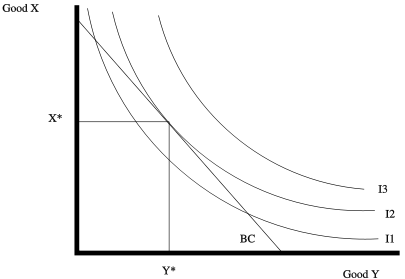
\includegraphics[scale=.35]{constraint.png}
\end{center}
\end{comment}

\textbf{Types of Constraints}: For a function \(f(x_1, \dots, x_n)\),
there are two types of constraints that can be imposed:

\begin{enumerate}
\item \textbf{Equality constraints:} constraints of the form $c(x_1,\dots, x_n) = r$.
Budget constraints are the classic example of equality constraints in social science.
\item \textbf{Inequality constraints:} constraints of the form $c(x_1, \dots, x_n) \leq r$.  These might arise from non-negativity constraints or other threshold effects.
\end{enumerate}

In any constrained optimization problem, the constrained maximum will
always be less than or equal to the unconstrained maximum. If the
constrained maximum is less than the unconstrained maximum, then the
constraint is binding. Essentially, this means that you can treat your
constraint as an equality constraint rather than an inequality
constraint.

For example, the budget constraint binds when you spend your entire
budget. This generally happens because we believe that utility is
strictly increasing in consumption, i.e.~you always want more so you
spend everything you have.

Any number of constraints can be placed on an optimization problem. When
working with multiple constraints, always make sure that the set of
constraints are not pathological; it must be possible for all of the
constraints to be satisfied simultaneously.

\textbf{Set-up for Constrained Optimization:}
\[\max_{x_1,x_2} f(x_1,x_2) \text{ s.t. } c(x_1,x_2)\]
\[\min_{x_1,x_2} f(x_1,x_2) \text{ s.t. } c(x_1,x_2)\] This tells us to
maximize/minimize our function, \(f(x_1,x_2)\), with respect to the
choice variables, \(x_1,x_2\), subject to the constraint.

Example:
\[\max_{x_1,x_2} f(x_1, x_2) = -(x_1^2 + 2x_2^2) \text{ s.t. }x_1 + x_2 = 4\]
It is easy to see that the \textit{unconstrained} maximum occurs at
\((x_1, x_2) = (0,0)\), but that does not satisfy the constraint. How
should we proceed?

\section{Equality Constraints}\label{equality-constraints}

Equality constraints are the easiest to deal with because we know that
the maximum or minimum has to lie on the (intersection of the)
constraint(s).

The trick is to change the problem from a constrained optimization
problem in \(n\) variables to an unconstrained optimization problem in
\(n + k\) variables, adding \textit{one} variable for \textit{each}
equality constraint. We do this using a lagrangian multiplier.

\textbf{Lagrangian function}: The Lagrangian function allows us to
combine the function we want to optimize and the constraint function
into a single function. Once we have this single function, we can
proceed as if this were an \textit{unconstrained} optimization
problem.\textbackslash{}

For each constraint, we must include a \textbf{Lagrange multiplier}
(\(\lambda_i\)) as an additional variable in the analysis. These terms
are the link between the constraint and the Lagrangian
function.\textbackslash{}

Given a \textit{two dimensional} set-up:
\[\max_{x_1,x_2}/\min_{x_1,x_2} f(x_1,x_2) \text{ s.t. } c(x_1,x_2) = a\]

We define the Lagrangian function \(L(x_1,x_2,\lambda_1)\) as follows:
\[L(x_1,x_2,\lambda_1) = f(x_1,x_2) - \lambda_1 (c(x_1,x_2) - a)\]

More generally, in \textit{n dimensions}:
\[ L(x_1, \dots, x_n, \lambda_1, \dots, \lambda_k) = f(x_1, \dots, x_n) - \sum_{i=1}^k\lambda_i(c_i(x_1,\dots, x_n) - r_i)\]

\textbf{Getting the sign right:}\textbackslash{} Note that above we
subtract the lagrangian term \textit{and} we subtract the constraint
constant from the constraint function. Occasionally, you may see the
following alternative form of the Lagrangian, which is
\textit{equivalent}:
\[ L(x_1, \dots, x_n, \lambda_1, \dots, \lambda_k) = f(x_1, \dots, x_n) + \sum_{i=1}^k\lambda_i(r_i - c_i(x_1,\dots, x_n))\]
Here we add the lagrangian term \textit{and} we subtract the constraing
function from the constraint constant.

\textbf{Using the Lagrangian to Find the Critical Points}: To find the
critical points, we take the partial derivatives of lagrangian function,
\(L(x_1, \dots, x_n, \lambda_1, \dots, \lambda_k)\), with respect to
each of its variables (all choice variables \({\bf x}\) \textit{and} all
lagrangian multipliers \({\bf \lambda}\)). At a critical point,
\textit{each} of these partial derivatives must be equal to zero, so we
obtain a system of \textit{$n + k$ equations in $n + k$ unknowns}:

\begin{eqnarray*}
\frac{\partial L}{\partial x_1} = \frac{\partial f}{\partial x_1} - \sum_{i = 1}^k\lambda_i\frac{\partial c_i}{\partial x_1} & = & 0\\
 \vdots & = & \vdots \nonumber \\ 
\frac{\partial L}{\partial x_n}  = \frac{\partial f}{\partial x_n} - \sum_{i = 1}^k\lambda_i\frac{\partial c_i}{\partial x_n} & =  & 0\\
\frac{\partial L}{\partial \lambda_1} = c_1(x_i, \dots, x_n) - r_1& = & 0\\
 \vdots & = & \vdots \nonumber \\
\frac{\partial L}{\partial \lambda_k} = c_k(x_i, \dots, x_n) - r_k & = & 0
\end{eqnarray*}

We can then solve this system of equations, because there are \(n+k\)
equations and \(n+k\) unknowns, to calculate the critical point
\((x_1^*,\dots,x_n^*,\lambda_1^*,\dots,\lambda_k^*)\).

\textbf{Second-order Conditions and Unconstrained Optimization:} There
may be more than one critical point, i.e.~we need to verify that the
critical point we find is a maximum/minimum. Similar to unconstrained
optimization, we can do this by checking the second-order conditions.

Example:\\
\[\max_{x_1,x_2} f(x) = -(x_1^2 + 2x_2^2) \text{ s.t. } x_1 + x_2 = 4\]

\begin{enumerate}
\item Begin by writing the Lagrangian:
$$L(x_1, x_2, \lambda) =  \phantom{-(x_1^2 + 2x_2^2) - \lambda(x_1 + x_2 - 4)}$$
\item Take the partial derivatives and set equal to zero:

\begin{eqnarray*}
\frac{\partial L}{\partial x_1} = \phantom{-2x_1 - \lambda} \quad \quad \quad & = & 0\\
\frac{\partial L}{\partial x_2}  = \phantom{-4x_2 - \lambda} \quad \quad \quad & =  & 0\\
\frac{\partial L}{\partial \lambda} = \phantom{-(x_1 + x_2 - 4)} \quad & = & 0\\
\end{eqnarray*}

\item Solve the system of equations:
\phantom{
1.  Using the first two partials, we see that $\lambda = -2x_1$ and $\lambda = -4x_2$\\
2.  Set these equal to see that $x_1 = 2x_2$\\
3.  Using the third partial and the above equality, $4 = 2x_2 + x_2 \Rightarrow x_2^* = 4/3$\\
4.  $\Rightarrow x_1^* = 8/3$ and $\lambda = -16/3$\\
5.  Therefore, the only critical point is $x_1^* = \frac{8}{3}$ and $x_2^* = \frac{4}{3}$\\
6. This gives $f(\frac{8}{3}, \frac{4}{3}) = -\frac{96}{9}$, which is less than the unconstrained optimum $f(0,0) = 0$}
\vspace{10pt}
\end{enumerate}

Notice that when we take the partial derivative of L with respect to the
lagranigian multiplier and set it equal to 0, we return exactly our
constraint! This is why signs matter.

\section{Inequality Constraints}\label{inequality-constraints}

Inequality constraints define the boundary of a region over which we
seek to optimize the function. This makes inequality constraints more
challenging because we do not know if the maximum/minimum lies along one
of the constraints (the constraint binds) or in the interior of the
region.

We must introduce more variables in order to turn the problem into an
unconstrained optimization.

\textbf{Slack:} For \textit{each} inequality constraint
\(c_i(x_1, \dots, x_n) \leq a_i\), we define a slack variable \(s_i^2\)
for which the expression \(c_i(x_1, \dots, x_n) \leq a_i - s_i^2\) would
hold with equality. These slack variables capture how close the
constraint comes to binding. We use \(s^2\) rather than \(s\) to ensure
that the slack is positive.

Slack is just a way to transform our constraints.

Given a \textit{two-dimensional} set-up and these edited constraints:
\[\max_{x_1,x_2}/\min_{x_1,x_2} f(x_1,x_2) \text{ s.t. } c(x_1,x_2) \le a_1\]

Adding in Slack:
\[\max_{x_1,x_2}/\min_{x_1,x_2} f(x_1,x_2) \text{ s.t. } c(x_1,x_2) \le a_1 - s_1^2\]

We define the Lagrangian function \(L(x_1,x_2,\lambda_1,s_1)\) as
follows:
\[L(x_1,x_2,\lambda_1,s_1) = f(x_1,x_2) - \lambda_1 ( c(x_1,x_2) + s_1^2 - a_1)\]

More generally, in \textit{n dimensions}:
\[ L(x_1, \dots, x_n, \lambda_1, \dots, \lambda_k, s_1, \dots, s_k) = f(x_1, \dots, x_n) - \sum_{i = 1}^k \lambda_i(c_i(x_1,\dots, x_n) + s_i^2 - a_i)\]

\textbf{Finding the Critical Points}: To find the critical points, we
take the partial derivatives of the lagrangian function,
\(L(x_1,\dots,x_n,\lambda_1,\dots,\lambda_k,s_1,\dots,s_k)\), with
respect to each of its variables (all choice variables \(x\), all
lagrangian multipliers \(\lambda\), and all slack variables \(s\)). At a
critical point, \textit{each} of these partial derivatives must be equal
to zero, so we obtain a system of
\textit{$n + 2k$ equations in $n + 2k$ unknowns}:

\begin{eqnarray*}
\frac{\partial L}{\partial x_1} = \frac{\partial f}{\partial x_1} - \sum_{i = 1}^k\lambda_i\frac{\partial c_i}{\partial x_1} & = & 0\\
 \vdots & = & \vdots \nonumber \\
\frac{\partial L}{\partial x_n}  = \frac{\partial f}{\partial x_n} - \sum_{i = 1}^k\lambda_i\frac{\partial c_i}{\partial x_n} & =  & 0\\
\frac{\partial L}{\partial \lambda_1} = c_1(x_i, \dots, x_n) + s_1^2 - b_1& = & 0\\
 \vdots & = & \vdots \nonumber \\
\frac{\partial L}{\partial \lambda_k} = c_k(x_i, \dots, x_n) + s_k^2 - b_k & = & 0\\
\frac{\partial L}{\partial s_1} = 2s_1\lambda_1 & = & 0\\
 \vdots & = & \vdots \nonumber \\
\frac{\partial L}{\partial s_k} = 2s_k\lambda_k & = & 0
\end{eqnarray*}

\textbf{Complementary slackness conditions}: The last set of first order
conditions of the form \(2s_i\lambda_i = 0\) (the partials taken with
respect to the slack variables) are known as complementary slackness
conditions. These conditions can be satisfied one of three ways:

\begin{enumerate}
\item $\lambda_i = 0$ and $s_i \neq 0$: This implies that the slack is positive and thus \textit{the constraint does not bind}.
\item $\lambda_i \neq 0$ and $s_i = 0$: This implies that there is no slack in the constraint and \textit{the constraint does bind}.
\item $\lambda_i = 0$ and $s_i = 0$: In this case, there is no slack but the \textit{constraint binds trivially}, without changing the optimum.\\
\end{enumerate}

Example: Find the critical points for the following constrained
optimization:
\[\max_{x_1,x_2} f(x) = -(x_1^2 + 2x_2^2) \text{ s.t. } x_1 + x_2 \le 4\]

\begin{enumerate}
\item Rewrite with the slack variables:
$$\max_{x_1,x_2} f(x) = -(x_1^2 + 2x_2^2) \text{ s.t. } x_1 + x_2 \le 4 - s_1^2$$

\item Write the Lagrangian:
$$L(x_1,x_2,\lambda_1,s_1) = -(x_1^2 + 2x_2^2) - \lambda_1 (x_1 + x_2 + s_1^2 - 4)$$

\item Take the partial derivatives and set equal to 0:

\begin{eqnarray*}
\frac{\partial L}{\partial x_1} = -2x_1 - \lambda_1  & = & 0\\
\frac{\partial L}{\partial x_2}  = -4x_2 - \lambda_1 & =  & 0\\
\frac{\partial L}{\partial \lambda_1} = -(x_1 + x_2 + s_1^2 - 4)& = & 0\\
\frac{\partial L}{\partial s_1} = -2s_1\lambda_1 & = & 0\\
\end{eqnarray*}

\item Consider all ways that the complementary slackness conditions are solved:
\begin{center}
\begin{tabular}{|l|cccc|c|}
\hline
Hypothesis & $s_1$ & $\lambda_1$ & $x_1$ & $x_2$ & $f(x_1, x_2)$\\
\hline
$s_1 = 0$ $\lambda_1 = 0$ & \multicolumn{4}{l|}{No solution} & \\
$s_1 \neq 0$ $\lambda_1 = 0$ & 2 & 0 & 0 & 0  & 0\\
$s_1 = 0$ $\lambda_1 \neq 0$ & 0 & $\frac{-16}{3}$ & $\frac{8}{3}$ & $\frac{4}{3}$ & $-\frac{32}{3}$\\
$s_1 \neq 0$ $\lambda_1 \neq 0$ & \multicolumn{4}{l|}{No solution} &\\
\hline
\end{tabular}
\end{center}

This shows that there are two critical points: $(0,0)$ and $(\frac{8}{3},\frac{4}{3})$.

\item Find maximum:
Looking at the values of $f(x_1,x_2)$ at the critical points, we see that $f(x_1,x_2)$ is maximized at $x_1^* = 0$ and $x_2^*=0$.

\end{enumerate}

Example: Find the critical points for the following constrained
optimization: \[\max_{x_1,x_2} f(x) = -(x_1^2 + 2x_2^2) \text{ s.t. } 
\begin{array}{l}
x_1 + x_2 \le 4\\
x_1 \ge 0\\
x_2 \ge 0
\end{array}\]

\begin{enumerate}
\item Rewrite with the slack variables:
$$\phantom{max_{x_1,x_2} f(x) = -(x_1^2 + 2x_2^2) \text{ s.t. } 
\begin{array}{l}
x_1 + x_2 \le 4 - s_1^2\\
-x_1 \le 0 - s_2^2\\
-x_2 \le 0 - s_3^2
\end{array}}$$

\item Write the Lagrangian:
$$\phantom{L(x_1, x_2, \lambda_1, \lambda_2, \lambda_3, s_1, s_2, s_3) =  -(x_1^2 + 2x_2^2) - \lambda_1(x_1 + x_2 + s_1^2  - 4) - \lambda_2(-x_1 + s_2^2) - \lambda_3(-x_2 + s_3^2)}$$
\item Take the partial derivatives and set equal to zero:
 
 \phantom{
$\frac{\partial L}{\partial x_1} = -2x_1 - \lambda_1 + \lambda_2  =  0$\\
$\frac{\partial L}{\partial x_2}  = -4x_2 - \lambda_1 + \lambda_3  =   0$\\
$\frac{\partial L}{\partial \lambda_1} = -(x_1 + x_2 + s_1^2 - 4) =  0$\\
$\frac{\partial L}{\partial \lambda_2} = -(-x_1 + s_2^2)  =  0$\\
$\frac{\partial L}{\partial \lambda_3} = -(-x_2 + s_3^2)  =  0$\\
$\frac{\partial L}{\partial s_1} = 2s_1\lambda_1  =  0$\\
$\frac{\partial L}{\partial s_2} = 2s_2\lambda_2  =  0$\\
$\frac{\partial L}{\partial s_3} = 2s_3\lambda_3  =  0$}
\item[]
\item[]
\item[]
\item[]
\item[]
\item[]
\item[]
\item[]
\item[]
\item[]
\item[]

\item Consider all ways that the complementary slackness conditions are solved:
\begin{center}
\begin{tabular}{|l|cccccccc|c|}
\hline
Hypothesis & $s_1$ & $s_2$ & $s_3$ & $\lambda_1$ & $\lambda_2$ & $\lambda_3$ & $x_1$ & $x_2$ & $f(x_1, x_2)$\\
\hline
$s_1 = s_2 = s_3 = 0$ & \multicolumn{8}{l|}{\phantom{No solution}} & \\
$s_1 \neq 0, s_2 = s_3 = 0$ & \phantom{2} & \phantom{0} & \phantom{0} & \phantom{0} & \phantom{0} & \phantom{0} & \phantom{0} & \phantom{0} & \phantom{0}\\
$s_2 \neq 0, s_1 = s_3 = 0$ & \phantom{0} & \phantom{2} & \phantom{0} & \phantom{-8} & \phantom{0} & \phantom{-8} & \phantom{4} & \phantom{0} & \phantom{-16}\\
$s_3 \neq 0, s_1 = s_2 = 0$ & \phantom{0} & \phantom{0} & \phantom{2} & \phantom{-16} & \phantom{-16} & \phantom{0} & \phantom{0} & \phantom{4} & \phantom{-32}\\
$s_1 \neq 0, s_2 \neq 0, s_3 = 0$ &\multicolumn{8}{l|}{\phantom{No solution}} & \\
$s_1 \neq 0, s_3 \neq 0, s_2 = 0$ &\multicolumn{8}{l|}{\phantom{No solution}} & \\
$s_2 \neq 0, s_3 \neq 0, s_1 = 0$ &\phantom{0} & \phantom{$\sqrt{\frac{8}{3}}$} & \phantom{$\sqrt{\frac{4}{3}}$} & \phantom{$-\frac{16}{3}$} & \phantom{0} & \phantom{0} & \phantom{$\frac{8}{3}$}& \phantom{$\frac{4}{3}$} & \phantom{$-\frac{32}{3}$}\\
$s_1 \neq 0, s_2 \neq 0, s_3 \neq 0$ &\multicolumn{8}{l|}{\phantom{No solution}}& \\
\hline
\end{tabular}
\end{center}

\phantom{This shows that there are four critical points: $(0,0)$, $(4,0)$, $(0,4)$, and $(\frac{8}{3},\frac{4}{3})$}

\item  Find maximum: \phantom{Looking at the values of $f(x_1,x_2)$ at the critical points, we see that the constrained maximum is located at $(x_1, x_2) = (0,0)$, which is the same as the unconstrained max.  The constrained minimum is located at $(x_1, x_2) = (0,4)$, while there is no unconstrained minimum for this problem.}

\end{enumerate}

\section{Kuhn-Tucker Conditions}\label{kuhn-tucker-conditions}

As you can see, this can be a pain. When dealing explicitly with
\textit{non-negativity constraints}, this process is simplified by using
the Kuhn-Tucker method.

\textbf{\bf Kuhn-Tucker conditions}: Because the problem of maximizing a
function subject to inequality and non-negativity constraints arises
frequently in economics, the Kuhn-Tucker approach provides a method that
often makes it easier to both calculate the critical points and identify
points that are (local) maxima.\textbackslash{}

Given a \textit{two-dimensional set-up}:
\[\max_{x_1,x_2}/\min_{x_1,x_2} f(x_1,x_2) \text{ s.t. }
\begin{array}{l}
c(x_1,x_2) \le a_1\\
x_1 \ge 0 \\
gx_2 \ge 0
\end{array}\]

We define the Lagrangian function \(L(x_1,x_2,\lambda_1)\) the same as
if we did not have the non-negativity constraints:
\[L(x_1,x_2,\lambda_2) = f(x_1,x_2) - \lambda_1(c(x_1,x_2) - a_1)\]

More generally, in \textit{n dimensions}:
\[ L(x_1, \dots, x_n, \lambda_1, \dots, \lambda_k) = f(x_1, \dots, x_n) - \sum_{i=1}^k\lambda_i(c_i(x_1,\dots, x_n) - a_i)\]

\textbf{Kuhn-Tucker and Complementary Slackness Conditions}: To find the
critical points, we first calculate the \textbf{Kuhn-Tucker conditions}
by taking the partial derivatives of the lagrangian function,
\(L(x_1,\dots,x_n,\lambda_1,\dots,\lambda_k)\), with respect to each of
its variables (all choice variable s\(x\) and all lagrangian multipliers
\(\lambda\)) \underline{and} we calculate the
\textbf{complementary slackness conditions} by multiplying each partial
derivative by its respective variable \underline{and} include
\textbf{non-negativity conditions} for all variables (choice variables
\(x\) and lagrangian multipliers \(\lambda\)).\textbackslash{}

\textbf{Kuhn-Tucker Conditions}

\begin{eqnarray*}
\frac{\partial L}{\partial x_1} \leq 0, & \dots, & \frac{\partial L}{\partial x_n} \leq 0\\
\frac{\partial L}{\partial \lambda_1} \geq 0, & \dots, & \frac{\partial L}{\partial \lambda_m} \geq 0
\end{eqnarray*}

\textbf{Complementary Slackness Conditions}

\begin{eqnarray*}
x_1\frac{\partial L}{\partial x_1} = 0, & \dots, & x_n\frac{\partial L}{\partial x_n} = 0\\
\lambda_1\frac{\partial L}{\partial \lambda_1} = 0, & \dots, & \lambda_m \frac{\partial L}{\partial \lambda_m} = 0
\end{eqnarray*}

\textbf{Non-negativity Conditions}

\begin{eqnarray*}
x_1 \geq 0 & \dots & x_n \geq 0\\
\lambda_1 \geq 0 & \dots & \lambda_m \geq 0
\end{eqnarray*}

Note that some of these conditions are set equal to 0, while others are
set as inequalities!\textbackslash{}

Note also that to minimize the function \(f(x_1, \dots, x_n)\), the
simplest thing to do is maximize the function \(-f(x_1, \dots, x_n)\);
all of the conditions remain the same after reformulating as a
maximization problem.\textbackslash{}

There are additional assumptions (notably, f(x) is quasi-concave and the
constraints are convex) that are sufficient to ensure that a point
satisfying the Kuhn-Tucker conditions is a global max; if these
assumptions do not hold, you may have to check more than one point.

\textbf{Finding the Critical Points with Kuhn-Tucker Conditions}: Given
the above conditions, to find the critical points we solve the above
system of equations. To do so, we must check \textit{all} border and
interior solutions to see if they satisfy the above conditions.

In a two-dimensional set-up, this means we must check the following
cases:

\begin{enumerate}
\item[(1)] \parbox[c]{2in}{$x_1 = 0, x_2 = 0$} \parbox{2in}{Border Solution}
\item[(2)] \parbox[c]{2in}{$x_1 = 0, x_2 \neq 0$} \parbox{2in}{Border Solution}
\item[(3)] \parbox[c]{2in}{$x_1 \neq 0, x_2 = 0$} \parbox{2in}{Border Solution}
\item[(4)] \parbox[c]{2in}{$x_1 \neq 0, x_2 \neq 0$} \parbox{2in}{Interior Solution}\\
\end{enumerate}

Example: \[\max_{x_1,x_2} f(x) = -(x_1^2 + 2x_2^2) \text{ s.t. } 
\begin{array}{l}
x_1 + x_2 \le 4\\
x_1 \ge 0\\
x_2 \ge 0
\end{array}\]

\begin{enumerate}
\item Write the Lagrangian:
$$L(x_1, x_2, \lambda) =  -(x_1^2 + 2x_2^2) - \lambda(x_1 + x_2 - 4)$$

\item Find the First Order Conditions:\\
Kuhn-Tucker Conditions
 \begin{eqnarray*}
\frac{\partial L}{\partial x_1} = -2x_1 - \lambda  & \leq & 0\\
\frac{\partial L}{\partial x_2}  = -4x_2 - \lambda & \leq  & 0\\
\frac{\partial L}{\partial \lambda} = -(x_1 + x_2 - 4)& \geq & 0
\end{eqnarray*}

Complementary Slackness Conditions
\begin{eqnarray*}
x_1\frac{\partial L}{\partial x_2} = x_1(-2x_1 - \lambda)  = & 0\\
x_2\frac{\partial L}{\partial x_2} = x_2(-4x_2 - \lambda)  & = & 0\\
\lambda\frac{\partial L}{\partial \lambda} = -\lambda(x_1 + x_2 - 4)& = & 0
\end{eqnarray*}

Non-negativity Conditions
\begin{eqnarray*}
x_1 & \geq & 0\\
x_2 & \geq & 0\\
\lambda & \geq & 0
\end{eqnarray*}

\item Consider all border and interior cases:
\begin{center}
\begin{tabular}{|l|ccc|c|}
\hline
Hypothesis  & $\lambda$& $x_1$ & $x_2$ & $f(x_1, x_2)$\\
\hline
$x_1 = 0, x_2 = 0$  &0 & 0 & 0 & 0\\
$x_1 = 0, x_2 \neq 0$  &-16 & 0 & 4 & -32\\
$x_1 \neq 0, x_2 = 0$  &-8 & 4 & 0 & -16\\
$x_1 \neq 0, x_2 \neq 0$ & $-\frac{16}{3}$ & $\frac{8}{3}$ & $\frac{4}{3}$ & $-\frac{32}{3}$\\
\hline
\end{tabular}
\end{center}

\item  Find Maximum:\\
Three of the critical points violate the requirement that $\lambda \geq 0$, so the point $(0,0,0)$ is the maximum.\\
\end{enumerate}

Example:

\[\max_{x_1,x_2} f(x) = \frac{1}{3}\log (x_1 + 1) + \frac{2}{3}\log (x_2 + 1) \text{ s.t. }  
\begin{array}{l}
x_1 + 2x_2 \leq 4\\
     x_1 \geq 0\\
    x_2 \geq 0
\end{array}\]

\begin{enumerate}
\item Write the Lagrangian:
$$\phantom{L(x_1, x_2, \lambda) =  \frac{1}{3}\log(x_1+1) + \frac{2}{3}\log(x_2+1) - \lambda(x_1 + 2x_2 - 4)}$$

\item Find the First Order Conditions:\\
Kuhn-Tucker Conditions\\
\phantom{$\frac{\partial L}{\partial x_1} = \frac{1}{3(x_1+1)} - \lambda   \leq  0$\\
$\frac{\partial L}{\partial x_2}  = \frac{2}{3(x_2+1)} - \lambda  \leq   0$\\
$\frac{\partial L}{\partial \lambda} = -(x_1 + 2x_2 - 4) \geq  0$}\\
\item[]
\item[]
\item[]
\item[]
\item[]
\item[]
\item[]
\item[]
 
Complementary Slackness Conditions\\
\phantom{$x_1\frac{\partial L}{\partial x_2} = x_1(\frac{1}{3(x_1+1)} - \lambda)  =  0$\\
$x_2\frac{\partial L}{\partial x_2} = x_2(\frac{2}{3(x_2+1)} - \lambda)   =  0$\\
$\lambda\frac{\partial L}{\partial \lambda} = -\lambda(x_1 + 2x_2 - 4) =  0$}\\
\item[]
\item[]
\item[]
\item[]
\item[]
\item[]
\item[]
\item[]
\item[]

Non-negativity Conditions\\
\phantom{$x_1  \geq  0$\\
$x_2  \geq  0$\\
$\lambda  \geq  $0}\\
\item[]
\item[]
\item[]

\item Consider all border and interior cases:
\begin{center}
\begin{tabular}{|l|ccc|c|}
\hline
Hypothesis  & $\lambda$& $x_1$ & $x_2$ & $f(x_1, x_2)$\\
\hline
$x_1 = 0, x_2 = 0$  &\multicolumn{3}{l|}{\phantom{No Solution}}& \\
$x_1 = 0, x_2 \neq 0$  &\multicolumn{3}{l|}{\phantom{No Solution}}& \\
$x_1 \neq 0, x_2 = 0$  & \multicolumn{3}{l|}{\phantom{No Solution}}& \\
$x_1 \neq 0, x_2 \neq 0$ &  & \phantom{$\frac{4}{3}$} & \phantom{$\frac{4}{3}$} & \phantom{$\log\frac{7}{3}$}\\
\hline
\end{tabular}
\end{center}

\item[]
\item[]
\item[]
\item[]

\item  Find Maximum:\\
\phantom{Three of the critical points violate the constraints, so the point $(\frac{4}{3},\frac{4}{3})$ is the maximum.}\\
\end{enumerate}

\chapter{Introduction}\label{intro}

You can label chapter and section titles using \texttt{\{\#label\}}
after them, e.g., we can reference Chapter \ref{intro}. If you do not
manually label them, there will be automatic labels anyway, e.g.,
Chapter \ref{methods}.

Figures and tables with captions will be placed in \texttt{figure} and
\texttt{table} environments, respectively.

\begin{Shaded}
\begin{Highlighting}[]
\KeywordTok{par}\NormalTok{(}\DataTypeTok{mar =} \KeywordTok{c}\NormalTok{(}\DecValTok{4}\NormalTok{, }\DecValTok{4}\NormalTok{, .}\DecValTok{1}\NormalTok{, .}\DecValTok{1}\NormalTok{))}
\KeywordTok{plot}\NormalTok{(pressure, }\DataTypeTok{type =} \StringTok{'b'}\NormalTok{, }\DataTypeTok{pch =} \DecValTok{19}\NormalTok{)}
\end{Highlighting}
\end{Shaded}

\begin{figure}

{\centering 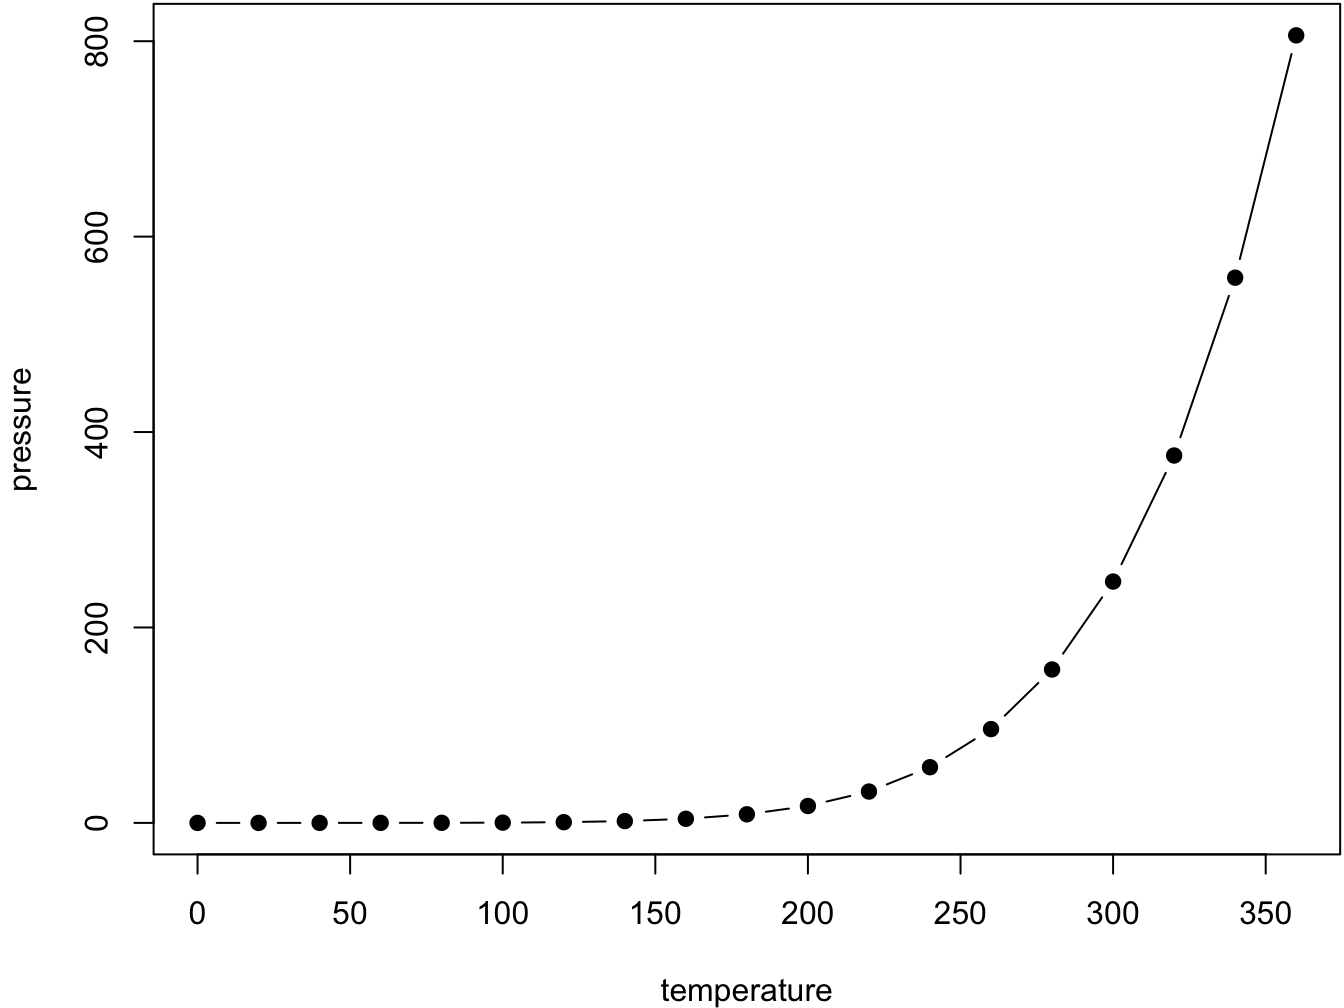
\includegraphics[width=0.8\linewidth]{prefresher_files/figure-latex/nice-fig-1} 

}

\caption{Here is a nice figure!}\label{fig:nice-fig}
\end{figure}

Reference a figure by its code chunk label with the \texttt{fig:}
prefix, e.g., see Figure \ref{fig:nice-fig}. Similarly, you can
reference tables generated from \texttt{knitr::kable()}, e.g., see Table
\ref{tab:nice-tab}.

\begin{Shaded}
\begin{Highlighting}[]
\NormalTok{knitr}\OperatorTok{::}\KeywordTok{kable}\NormalTok{(}
  \KeywordTok{head}\NormalTok{(iris, }\DecValTok{20}\NormalTok{), }\DataTypeTok{caption =} \StringTok{'Here is a nice table!'}\NormalTok{,}
  \DataTypeTok{booktabs =} \OtherTok{TRUE}
\NormalTok{)}
\end{Highlighting}
\end{Shaded}

\begin{table}

\caption{\label{tab:nice-tab}Here is a nice table!}
\centering
\begin{tabular}[t]{rrrrl}
\toprule
Sepal.Length & Sepal.Width & Petal.Length & Petal.Width & Species\\
\midrule
5.1 & 3.5 & 1.4 & 0.2 & setosa\\
4.9 & 3.0 & 1.4 & 0.2 & setosa\\
4.7 & 3.2 & 1.3 & 0.2 & setosa\\
4.6 & 3.1 & 1.5 & 0.2 & setosa\\
5.0 & 3.6 & 1.4 & 0.2 & setosa\\
\addlinespace
5.4 & 3.9 & 1.7 & 0.4 & setosa\\
4.6 & 3.4 & 1.4 & 0.3 & setosa\\
5.0 & 3.4 & 1.5 & 0.2 & setosa\\
4.4 & 2.9 & 1.4 & 0.2 & setosa\\
4.9 & 3.1 & 1.5 & 0.1 & setosa\\
\addlinespace
5.4 & 3.7 & 1.5 & 0.2 & setosa\\
4.8 & 3.4 & 1.6 & 0.2 & setosa\\
4.8 & 3.0 & 1.4 & 0.1 & setosa\\
4.3 & 3.0 & 1.1 & 0.1 & setosa\\
5.8 & 4.0 & 1.2 & 0.2 & setosa\\
\addlinespace
5.7 & 4.4 & 1.5 & 0.4 & setosa\\
5.4 & 3.9 & 1.3 & 0.4 & setosa\\
5.1 & 3.5 & 1.4 & 0.3 & setosa\\
5.7 & 3.8 & 1.7 & 0.3 & setosa\\
5.1 & 3.8 & 1.5 & 0.3 & setosa\\
\bottomrule
\end{tabular}
\end{table}

You can write citations, too. For example, we are using the
\textbf{bookdown} package \citep{R-bookdown} in this sample book, which
was built on top of R Markdown and \textbf{knitr} \citep{xie2015}.

\bibliography{book.bib,packages.bib}


\end{document}
